\documentclass[a4paper,11pt]{article} \pdfoutput=1

\usepackage{jcappub}
\usepackage[T1]{fontenc}
\usepackage{physics}
\usepackage{bm}
\usepackage{subcaption}
\usepackage{tikz-feynman}
\newcommand{\rhn}{\bar{\nu}}
\newcommand{\cA}{\mathcal{A}}
\newcommand{\cB}{\mathcal{B}}
\newcommand{\cC}{\mathcal{C}}
\newcommand{\cD}{\mathcal{D}}
\newcommand{\cV}{\mathcal{V}}
\newcommand{\cL}{\mathcal{L}}
\newcommand{\cN}{\mathcal{N}}
\newcommand{\cM}{\mathcal{M}}
\newcommand{\cK}{\mathcal{K}}
\newcommand{\cJ}{\mathcal{J}}
\newcommand{\cS}{\mathcal{S}}
\newcommand{\OmegaVV}{\Omega_{\nu\nu}}
\newcommand{\OmegaVN}{\Omega_{\nu\rhn}}
\newcommand{\OmegaNV}{\Omega_{\rhn\nu}}
\newcommand{\OmegaNN}{\Omega_{\rhn\rhn}}

\newcommand{\OmegaVVb}{\bm{\Omega}_{\nu\nu}}
\newcommand{\OmegaVNb}{\bm{\Omega}_{\nu\rhn}}
\newcommand{\OmegaNVb}{\bm{\Omega}_{\rhn\nu}}
\newcommand{\OmegaNNb}{\bm{\Omega}_{\rhn\rhn}}

\newcommand{\ChiPT}{\mathrm{ChiPT}}

\newcommand{\cw}{{c_{W}}}
\newcommand{\sw}{{s_{W}}}
\newcommand{\fpi}{{f_{\pi}}}
\newcommand{\gf}{{G_{F}}}
\newcommand{\vud}{{V_{ud}}}
\newcommand{\vus}{{V_{us}}}
\newcommand{\vudc}{{V^{*}_{ud}}}
\newcommand{\vusc}{{V^{*}_{us}}}

\newcommand{\piz}{{\pi^{0}}}
\newcommand{\pip}{{\pi^{+}}}
\newcommand{\pim}{{\pi^{-}}}
\newcommand{\kp}{{K^{+}}}
\newcommand{\km}{{K^{-}}}
\newcommand{\kz}{{K^{0}}}
\newcommand{\kzb}{{\bar{K}^{0}}}

\newcommand{\si}{{\sigma}}
\newcommand{\sibar}{{\bar{\sigma}}}

\newcommand{\RefCite}[1]{Ref.~(\cite{#1})}
\newcommand{\FigRef}[1]{Fig.~(\ref{#1})}
\newcommand{\EqnRef}[1]{Eqn.~(\ref{#1})}
\newcommand{\TabRef}[1]{Eqn.~(\ref{#1})}

\tikzfeynmanset{
	warn luatex=false
}


\title{\boldmath Indirect Detection Signatures of Dark Matter Annihilation/Decay to Right-Handed Neutrinos}

%% %simple case: 2 authors, same institution
%% \author{A. Uthor}
%% \author{and A. Nother Author}
%% \affiliation{Institution,\\Address, Country}

% more complex case: 4 authors, 3 institutions, 2 footnotes
\author[a,b,1]{Stefania Gori}
\author[a,b]{Logan Morrison}
\author[a,b]{Stefano Profumo}
\author[c,d]{Bibhushan Shakya}

\affiliation[a]{Department of Physics, 1156 High St., University of California Santa Cruz, Santa Cruz, CA 95064, USA}
\affiliation[b]{Santa Cruz Institute for Particle Physics, 1156 High St., Santa Cruz, CA 95064, USA}
\affiliation[c]{DESY, Notkestrasse 85, 22607 Hamburg, Germany}
\affiliation[d]{CERN, Theoretical Physics Department, 1211 Geneva 23, Switzerland}

% e-mail addresses: one for each author, in the same order as the authors
\emailAdd{sgori@ucsc.edu}
\emailAdd{loanmorr@ucsc.edu}
\emailAdd{profumo@ucsc.edu}
\emailAdd{bibhushan.shakya@desy.de}




\abstract{Very much so.}



\begin{document}
\maketitle
\flushbottom

\section{Overview}\label{sec:intro}
Right handed neutrinos (RHN), also referred to as sterile neutrinos or heavy
neutral leptons, are one of the most well-motivated extensions to the Standard
Model, featuring in many models of neutrino mass generation. In such models,
RHNs are often part of an extended sector that also contains dark matter. Such
frameworks have been extensively studied in the literature under the broad
umbrella of neutrino portal dark matter
\cite{Falkowski:2009yz,Macias:2015cna,Escudero:2016ksa,Escudero:2016tzx,Tang:2016sib,Batell:2017cmf,Batell:2017rol,Shakya:2018qzg,Patel:2019zky},
where the RHNs act as the portal connecting dark matter to the visible sector.

If sterile neutrinos are heavier, dark matter annihilates or decays directly to
SM neutrinos via the mixing between the sterile and active neutrinos (see e.g.
\cite{Falkowski:2009yz,Patel:2019zky}). On the other hand, if dark matter is
heavier than the RHNs, dark matter annihilates or decays exclusively to RHNs,
and subsequent decays of the RHNs into SM particles then give rise to visible
signals. Such signals have been employed in the past to explain various
putative dark matter signals such as the Galactic Center excess
\cite{Tang:2015coo} and high energy neutrinos at IceCube \cite{Roland:2015yoa}.
Such signals are fairly insensitive to the exact nature of the underlying
model, since dark matter annihilations (or decays) produce an isotropic
distribution of RHNs with energy $m_{DM}(\text{or }m_{DM}/2)$. The decay
lifetimes of the RHNs are constrained by the seesaw mechanism and can generally
be considered prompt on astrophysical scales (exceptional cases occur when
considering dark matter annihilation/decay in the sun
\cite{Allahverdi:2016fvl}, or RHNs with extremely long lifetimes
\cite{Gori:2018lem}). Therefore, the spectra of visible signals (in photons,
neutrinos, charged leptons, antiprotons) are essentially determined by only two
parameters: the dark matter mass $m_{DM}$ and the right handed neutrino mass
$m_{N}$.  The goal of our paper is to perform an extensive study of such
signals in terms of these parameters. Indirect detection signals of dark matter
annihilation into right handed neutrinos have been studied for specific cases:
for $m_N=1-5$ GeV in \cite{Allahverdi:2016fvl}, and for $m_N=10-1000$ GeV in
\cite{Campos:2017odj}.

\section{Framework}
\label{sec:framework}

Effective operator between dark matter $X$ and RHNs $N$ facilitate either
annihilations or decays. $N$ couples to the SM via Dirac mass term $LHN$.
Everything follows from this.

We consider two dark matter models: one in which the dark matter decays into
two RH neutrinos and another where the dark matter annihilates into RH
neutrinos. For the purposes of this paper, the exact form of the interactions
are irrelevent; we need only assume that they exist and produce either \(\chi
\to \rhn\rhn\) or \(\chi\bar{\chi} \to \rhn\rhn\). The shapes of the spectra we
will present do not depend on the specifics of the interactions since the
energy of the final-state RH neutrinos (which in turn dictates the decay
spectra) only depends on the center-of-mass energy of the process which is
fixed by the dark matter mass and velocity. Thus, for the remainder of this section
we will focus on the RH neutrino interactions with the SM.

We assume the existance of a single Majorana RH which couples to the SM via a
Yukawa interaction. In two-component spinor notation, the terms in the
Lagrangian density containing the neutrinos are:
\begin{align}
	\mathcal{L}
	 & \supset
	i\hat{\rhn}^{\dagger}\bar{\sigma}_{\mu}\partial^{\mu}\hat{\rhn}
	- \frac{1}{2}\hat{m}_{\hat{\rhn}}\qty(\hat{\rhn}\hat{\rhn} + \hat{\rhn}^{\dagger}\hat{\rhn}^{\dagger})
	+ \epsilon^{ab}Y^{i}_{\nu}\Phi_{a}L_{bi}\hat{\rhn}
	- Y^{i}_{\ell}\Phi_{a}L_{bi}\hat{\nu}
\end{align}
Here, \(\epsilon^{ab}\) is two-dimensional Levi-Civita with \(\epsilon^{12}=+1\), \(\Phi_{a}\) is the Higgs doublet, \(L_{bi}\) is the lepton doublet for
the \(i\)th generation (assumed to be such that the charged lepton mass matrix is diagonal),
and \(\hat{\rhn}\) is the RH neutrino represented as a two-component
Majorana spinor. The vector \(Y^{i}_{\nu}\) is a Yukawa vector coupling the
\(i\)th lepton doublet to the RH neutrino. Expanding the Higgs around its vacuum
expectation value, the neutrino mass terms are:
\begin{align}
	\mathcal{L}_{\mathrm{mass},\nu}
	                        & \supset
	- \frac{1}{2}\hat{m}_{\hat{\rhn}}\qty(\hat{\rhn}\hat{\rhn} + \hat{\rhn}^{\dagger}\hat{\rhn}^{\dagger})
	- \frac{v}{\sqrt{2}}Y^{i}_{\nu}\hat{\nu}_{i}\hat{\rhn}
	=
	-\frac{1}{2}
	\mathcal{N}^{T}
	\mqty(\bm{0}_{3\times3} & \frac{v}{\sqrt{2}}Y_{\nu} \\ \frac{v}{\sqrt{2}}Y^{T}_{\nu} & \hat{m}_{\hat{\rhn}})
	\mathcal{N}
\end{align}
Here \(\mathcal{N} = \mqty(\hat{\nu}_1 & \hat{\nu}_3 &\hat{\nu}_3&\hat{\rhn})^{T}\)
is a vector composed of all neutrinos. For simplicity, we will assume that only
a single entry of \(Y_{\nu}\) is non-zero. We set \(Y^{k}_{\hat{\nu}} = y\)
and \(Y^{i}_{\hat{\nu}} = 0\) for \(i\neq k\). In this case, we may safely drop
the active neutrinos \(\hat{\nu}_{i}\) for \(i\neq k\) from mass matrix and
take them to be mass eigenstates. Then, our neutrino mass terms reduce to
\begin{align}
	\mathcal{L}_{\mathrm{mass},\nu}
	                    & \supset
	=
	-\frac{1}{2}
	\mqty(\hat{\nu}_{k} & \hat{\rhn})
	\underbrace{\mqty(0 & \frac{v}{\sqrt{2}}y \\ \frac{v}{\sqrt{2}}y & \hat{m}_{\hat{\rhn}})}_{M_{\nu}}
	\mqty(\hat{\nu}_{k}                       \\ \hat{\rhn})
\end{align}
The neutrino mass matrix can be diagonalized using Takagi diagonalization via a
unitary matrix \(\Omega\) where
\(\Omega^{T}M_{\nu}\Omega = \mathrm{diag}(m^{k}_{\nu}, m_{\rhn})\). The
explicit form of \(\Omega\) is:
\begin{align}
	\Omega = \mqty(-i\cos\theta & \sin\theta \\ i\sin\theta & \cos\theta)
\end{align}
which can easily be checked to be unitary. The parameters
\(y, \hat{m}_{\hat{\rhn}}\) can be translated to \(m_{\rhn}\) and \(\theta\)
given:
\begin{align}
	y & = \frac{\sqrt{2}m_{\rhn}\tan\theta}{v}, & \hat{m}_{\hat{\rhn}} & = m_{\rhn}\qty(1-\tan^2\theta).
\end{align}
In addition, the left-handed neutrino mass is \(m^{k}_{\nu} = m_{\rhn}\tan^2\theta\).
To obtain the interactions between the RH neutrino and SM particles, we use
\begin{align}\label{eqn:framework:gauge_to_mass_eigenstates}
	\hat{\nu}  & = -i\cos\theta\nu_{k} + \sin\theta\rhn, &
	\hat{\rhn} & = i\sin\theta\nu_{k} + \cos\theta\rhn,
\end{align}
where the unhatted fields \(\nu_{k}\) and \(\rhn\) are mass eigenstates.

Making the replacements given in Eqn.~\ref{eqn:framework:gauge_to_mass_eigenstates}, we find
the following interaction Lagrangian for the RH-neutrino and \(\nu_{k}\):
\begin{align}\label{eqn:framework:ew_interaction_lagrangian}
	\cL_{\mathrm{int},\nu} & =
	\cL_{\nu W^{\pm}}
	+ \cL_{\nu Z}
	+ \cL_{\nu h}
	+ \cL_{\nu G^{\pm}}
	+ \cL_{\nu G^{0}}
\end{align}
where the \(W\), \(Z\) and Higgs Lagrangians are
\begin{align}
	% KL = -I * Cos[theta]
	% KR = Sin[theta]
	% KL^d KL = Cos[theta]^2
	% KL^d KR = I*Cos[theta]*Sin[theta]
	% KR^d KL = -I*Cos[theta]*Sin[theta]
	% KR^d KR = Sin[theta]^2
	% KL.mv = I*mvr*Sin[theta]*Tan[theta]
	% KR.mn = mvr * Sin[theta]
	% Transpose[KL].Conjugate[KL].mv = mvr Sin[theta]^2
	% Transpose[KR].Conjugate[KR].mn = mvr Sin[theta]^2
	% Transpose[KL].Conjugate[KR].mn = -I mvr Cos[theta] Sin[theta]
	% Transpose[KR].Conjugate[KL].mv = I mvr Sin[theta]^2 Tan[theta]
	% ml.KL = -I me Cos[theta]
	% ml.KR = me Sin[theta]
	\cL_{\nu W^{\pm}}
	 & =
	\frac{e}{\sqrt{2}\sw}\qty(-i\cos\theta W^{-}_{\mu}\ell^{\dagger}_{k}\bar{\sigma}_{\mu}\nu_{k}
	+ \sin\theta W^{-}_{\mu}\ell^{\dagger}_{k}\bar{\sigma}_{\mu}\rhn) + \mathrm{h.c} \\
	%-----------
	\cL_{\nu Z}
	 & =
	\frac{e}{2\cw\sw}Z_{\mu}\qty[
		\cos^2\theta\nu^{\dagger}_{k}\bar{\sigma}_{\mu}\nu_{k}
		+ \sin^2\theta\rhn^{\dagger}\bar{\sigma}_{\mu}\rhn
		+ \qty(i\cos\theta\sin\theta \nu_{k}^{\dagger}\bar{\sigma}_{\mu}\rhn + \mathrm{c.c})
	]                                                                                \\
	%-----------
	\cL_{\nu h}
	 & =
	-\frac{h\sin\theta}{v}\qty[
		m_{\nu}\cos\theta\nu_{k}\nu_{k}
		+ m_{\rhn}\sin\theta\rhn\rhn
		+ \qty(i m_{\rhn}\cos\theta\rhn\nu_{k} + \mathrm{c.c.})
	] + \mathrm{c.c.}
\end{align}
and the Goldstone Lagrangians are
\begin{align}
	\cL_{\nu G^{\pm}}
	 & =
	\frac{\sqrt{2}G^{+}}{v}\ell_{k}\qty(
	im_{\nu}\sin\theta\nu_{k}
	+ m_{\rhn}\sin\theta\rhn)
	+ \frac{\sqrt{2}m_{\ell_{k}}G^{-}}{v}\bar{\ell}_{k}\qty(
	i\cos\theta\nu_{k}
	+ \sin\theta\rhn)
	+ \mathrm{c.c.}
	\\
	%-----------
	\cL_{\nu G^{0}}
	 & =
	-\frac{i G^{0}\sin\theta}{v}\qty[
		m_{\nu}\cos\theta\nu_{k}\nu_{k}
		+ m_{\rhn}\sin\theta\rhn\rhn
		+ \qty(i m_{\rhn}\cos\theta\rhn\nu_{k} + \mathrm{c.c.})
	] + \mathrm{c.c.}
\end{align}
In these Lagrangians, \(c_{W},s_{W}\) are the cosine and sine of the weak
mixing angle, \(e\) is the EM gauge coupling and ``\(\mathrm{c.c.}\)'' stands
for ``complex conjugate''.

The Lagrangian presented in Eqn.~\ref{eqn:framework:ew_interaction_lagrangian} is appropriate
for RH neutrino masses \(\gtrsim\) few GeV. For sub-GeV RH neutrino masses, we
need to integrate out the \(W\), \(Z\) and Higgs and match onto an effective
Lagrangian that takes into account QCD bound states. For this purpose, we use
the Chiral Lagrangian. We match onto the chiral Lagrangian in two steps: first
we integrate out the heavy bosons then we match the resulting Lagrangian onto
the chiral Lagrangian.

In this study, we will restrict ourselves to the leading-order chiral Lagrangian, which is given by:
\begin{align}
	\cL_{\ChiPT}
	 & =
	\frac{\fpi^{2}}{4}\Tr[\qty(D_{\mu}\bm{\Sigma})^{\dagger}\qty(D^{\mu}\bm{\Sigma})]
	+ \frac{\fpi^{2}}{4}\Tr[\bm{\Sigma}^{\dagger}\bm{\chi} + \bm{\chi}^{\dagger}\bm{\Sigma}]
\end{align}
where \(\fpi \sim 93\) MeV is the pion decay constant, \(\bm{\Sigma}\) is the
exponetial of the Psuedo-Goldstone matrix, \(D_{\mu}\) is the chiral covariant
derivate and \(\bm{\chi}\) is a Spurion field mediating the soft chiral
symmetry breaking. Explicitly, \(\bm{\Sigma}\) is given by:
\begin{align}
	\bm{\Sigma}              & = \exp(\frac{i}{\fpi}\phi^{a}\bm{\lambda}_{a}), &
	\phi^{a}\bm{\lambda}_{a} & =
	\mqty(
	\piz + \eta_{8}/\sqrt{3} & \sqrt{2}\pip                                    & \sqrt{2}\kp                 \\
	\sqrt{2}\pim             & -\piz +\eta_{8}/\sqrt{3}                        & \sqrt{2}\kz                 \\
	\sqrt{2}\km              & \sqrt{2}\kzb                                    & -\sqrt{\frac{2}{3}}\eta_{8} \\
	)
\end{align}
The chiral covariant derivative is given by
\begin{align}
	D_{\mu}\bm{\Sigma} & = \partial_{\mu}\bm{\Sigma} -i \bm{R}_{\mu}\bm{\Sigma} + i \bm{\Sigma}\bm{L}_{\mu}
\end{align}
with \(\bm{R}_{\mu}\) and \(\bm{L}_{\mu}\) representing the right and left
handed quark currents. The Spurion field \(\bm{\chi}\) is taken to have a
vacuum expectation value the breaks chiral symmetry breaking is the same
way that quark masses do:
\begin{align}
	\bm{\chi} & = 2B_{0}\qty(\bm{M}_{q} + \bm{s} + i\bm{p})
\end{align}
Here, \(B_{0}\) is related to the quark condensate via \(B_{0} \sim
-\expval{\bar{\bm{q}}\bm{q} + \bar{\bm{q}}^{\dagger}\bm{q}^{\dagger}} /
(3\fpi)\)\footnote{The \(B_{0}\) parameter is ultimately removed in favor of
the meson masses. For expample, we can use \(m_{\pi^{\pm}} =
B_{0}(m_{u}+m_{d})\).} and \(\bm{s}\) and \(\bm{p}\) are the scalar and
psuedo-scalar quark currents. The currents \(\bm{L}_{\mu}, \bm{R}_{\mu},
\bm{s}\) and \(\bm{p}\) are determined from the light-quark Lagrangian, written
as:
\begin{align}
	\cL =
	\cdots
	+ \bm{q}^{\dagger}\bm{L}^{\mu}\sibar_{\mu}\bm{q}
	+ \bar{\bm{q}}^{\dagger}\bm{R}^{\mu}\sibar_{\mu}\bar{\bm{q}}
	+ \bm{q}\qty(\bm{s}-i\bm{p})\bar{\bm{q}}
	+ \bm{q}^{\dagger}\qty(\bm{s}+i\bm{p})\bar{\bm{q}}^{\dagger}
\end{align}
where \(\bm{q}\) and \(\bar{\bm{q}}\) are the vectors containings the left and
right handed light quarks:
\begin{align}
	\bm{q}       & = \mqty(u       \\ d \\ s), &
	\bar{\bm{q}} & = \mqty(\bar{u} \\ \bar{d} \\ \bar{s}) .
\end{align}
Thus, matching onto the chiral Lagrangian simply requires us to identify the
quark currents.

To identify the quarks currents, we begin by integrating out the heavy bosons. The result is the well-known
4-Fermi Lagrangian, given by:
\begin{align}\label{eqn:framework:four_fermi}
	\cL_{4F} & = -\frac{4\gf}{\sqrt{2}}\qty[J^{+}_{\mu}J^{-}_{\mu} + J^{Z}_{\mu}J^{Z}_{\mu}]
\end{align}
where the charged and neutral currents are given by:
\begin{align}
	J^{+}_{\mu}     & = \hat{\nu}_{i}^{\dagger}\sibar_{\mu}\ell_{i} + V_{ud}u^{\dagger}\sibar_{\mu}d + V_{us}u^{\dagger}\sibar_{\mu}s         \\
	J^{-}_{\mu}     & = \ell_{i}^{\dagger}\sibar_{\mu}\hat{\nu}_{i} + V^{*}_{ud}d^{\dagger}\sibar_{\mu}u + V^{*}_{us}s^{\dagger}\sibar_{\mu}u \\
	\cw J^{Z}_{\mu} & =
	g_{L,\nu}\hat{\nu}_{i}^{\dagger}\sibar_{\mu}\hat{\nu}_{i}
	+ g_{L,\ell}\ell_{i}^{\dagger}\sibar_{\mu}\ell_{i}
	+ g_{R,\ell}\bar{\ell}_{i}^{\dagger}\sibar_{\mu}\bar{\ell}_{i}
	+ \sum_{q=u,d,s}\qty(
	g_{L,q}q^{\dagger}\bar{\sigma}_{\mu}q + g_{R,q}\bar{q}^{\dagger}\bar{\sigma}_{\mu}\bar{q})
\end{align}
where the sum over \(i\) is implied, \(V_{ud}\) and \(V_{us}\) are the \(u\)-\(d\)
and \(u\)-\(s\) CKM matrix elements, and the left/right-handed couplings are given by:
\begin{align}
	g_{L,u}    & = \frac{1}{2} - \frac{2}{3}\sw^2,  &
	g_{L,d}    & = -\frac{1}{2} + \frac{1}{3}\sw^2, &
	g_{L,\nu}  & = \frac{1}{2},                     &
	g_{L,\ell} & = -\frac{1}{2} + \sw^2,              \\
	%-------
	g_{R,u}    & = -\frac{2}{3}\sw^2,               &
	g_{R,d}    & = \frac{1}{3}\sw^2,                &
	g_{R,\ell} & = \sw^2 .
\end{align}
Expanding out Eqn.~\ref{eqn:framework:four_fermi}, it can be brought into the following
form:
\begin{align}
	-\frac{\sqrt{2}}{4\gf}\cL_{4F}
	 & =
	\bm{q}^{\dagger}\qty[\bm{V}j_{\mu}^{-} + \bm{V}^{\dagger}j_{\mu}^{+} + \frac{2}{\cw}\bm{G}_{L,q}j_{\mu}^{Z}]\sibar_{\mu}\bm{q}
	+ \frac{2}{\cw}\bar{\bm{q}}^{\dagger}\qty(\bm{G}_{R,q}j_{\mu}^{Z})\sibar_{\mu}\bar{\bm{q}} \\
	 & \quad
	+ j_{\mu}^{+}j_{\mu}^{-} + j_{\mu}^{Z}j_{\mu}^{Z}
	+ \cdots \notag
\end{align}
where the \(\cdots\) contain terms that contribute to the next to leading order
chiral Lagrangian and \(j^{\pm}_{\mu}\) and \(j^{Z}_{\mu}\) are the charged and neutral currents containing leptons only:
\begin{align}
	j^{+}_{\mu}
	                                             & =
	\hat{\nu}_{i}^{\dagger}\sibar_{\mu}\ell_{i}, &
	%-----
	j^{-}_{\mu}
	                                             & =
	\ell_{i}^{\dagger}\sibar_{\mu}\hat{\nu}_{i}      \\
	%----
	j^{Z}_{\mu}
	                                             & =
	g_{L,\nu}\hat{\nu}_{i}^{\dagger}\sibar_{\mu}\hat{\nu}_{i}
	+ g_{L,\ell}\ell_{i}^{\dagger}\sibar_{\mu}\ell_{i}
	+ g_{R,\ell}\bar{\ell}_{i}^{\dagger}\sibar_{\mu}\bar{\ell}_{i}
\end{align}
The coupling matrices \(\bm{V}\), \(\bm{G}_{L,q}\) and \(\bm{G}_{R,q}\)
are given by:
\begin{align}
	\bm{V}
	        & =
	\mqty(0 & V_{ud} & V_{us} \\ 0&0&0\\ 0&0&0),
	        &
	\bm{G}_{L,q}
	        & =
	\bm{T}_{3,q} - s_{W}^{2}\bm{Q}_{q},
	        &
	\bm{G}_{R,q}
	        & =
	-s_{W}^{2}\bm{Q}_{q}
\end{align}
with \(\bm{Q}_{q}\) the light-quark charge matrix and \(\bm{T}_{3,q}\) a matrix
containing the light-quark weak-isospin eigenvalues
\begin{align}
	\bm{Q}_{q}
	 & =
	\frac{1}{3}\mqty(\dmat{2,-1,-1}),
	 &
	\bm{T}_{3,q}
	 & =
	\frac{1}{2}\mqty(\dmat{1,-1,-1}),
\end{align}
Written in this form, we can immediately identify the left and right handed currents as:
\begin{align}
	\bm{L}_{\mu}
	 & =
	%-\frac{1}{3c_{W}}j^{Z}_{\mu}\bm{I}
	\frac{2(1-s_{W}^{2})}{c_{W}}\qty(\bm{\lambda}_{3}+\frac{1}{\sqrt{3}}\bm{\lambda}_{8})j^{Z}_{\mu}
	+
	\qty[
	\qty(
	V^{*}_{ud}\bm{\lambda}^{+}_{12} + V^{*}_{us}\bm{\lambda}^{+}_{45}
	)j^{+}_{\mu}
	+\mathrm{c.c.}
	]\notag \\
	\bm{R}_{\mu}
	 & =
	-\frac{2s_{W}^{2}}{c_{W}^{2}}
	\qty(\bm{\lambda}_{3}+\frac{1}{\sqrt{3}}\bm{\lambda}_{8})j^{Z}_{\mu}
\end{align}
where \(\bm{\lambda}^{\pm}_{12} = (\bm{\lambda}_{1} \mp i\bm{\lambda}_{2})/2\)
and \(\bm{\lambda}^{\pm}_{45} = (\bm{\lambda}_{4} \mp i\bm{\lambda}_{5})/2\).
Note that we have not included the singlet term of \(\bm{L}_{\mu}\) since the
vector singlet vanishes from the chiral covariant derivative and the axial
singlet must be taken into account via the chiral anomaly.

If we expand the chiral Lagrangian to order \(\gf\), we find the following Lagrangian:
\begin{align}
	\cL & =
	-\frac{4G_{F}}{\sqrt{2}}\qty(
	j^{Z}_{\mu}\cJ^{0}_{\mu}
	+ \qty(j^{+}_{\mu}\cJ^{+}_{0} + \mathrm{c.c.})
	+\qty(j^{Z}_{\mu})^{2}\cS^{0}
	+j^{Z}_{\mu}\qty(j^{+}_{\mu}\cS^{+}+\mathrm{c.c.})
	)
\end{align}
Here, the neutral meson current \(\cJ^{0}_{\mu}\) is given by:
\begin{align}
	\cJ^{0}_{\mu} & =
	\frac{f_{\pi}}{c_{W}}\qty[
		\partial^{\mu}\pi^{0}
		+ \frac{1}{\sqrt{3}}
		\partial^{\mu}\eta
	]
	- \frac{i (1-2s_{W}^{2})}{c_{W}}
	\qty[
	\pi^{+}\overleftrightarrow{\partial}_{\mu}\pi^{-} +
	K^{+}\overleftrightarrow{\partial}_{\mu}K^{-}
	]
\end{align}
where \(X\overleftrightarrow{\partial}_{\mu}Y \equiv X\partial_{\mu}Y - Y\partial_{\mu}X\).
The charged meson current is:
\begin{align}
	\cJ^{+}_{\mu}
	 & =
	\frac{f_{\pi}}{\sqrt{2}}\qty[
	V^{*}_{ud}\partial^{\mu}\pi^{+}
	+ V^{*}_{us}\partial^{\mu}K^{+}
	]
	\\
	 & \quad
	+ i
	\frac{V^{*}_{ud}}{2}\qty(
	\bar{K}^{0}\overleftrightarrow{\partial}_{\mu}K^{+}
	+ \sqrt{2}\pi^{+}\overleftrightarrow{\partial}_{\mu}\pi^{0}
	)\notag  \\
	 & \quad
	+i\frac{V_{us}^{*}}{2}\qty(
	K^{0}\overleftrightarrow{\partial}_{\mu}\pi^{+}
	+\sqrt{\frac{3}{2}}K^{+}\overleftrightarrow{\partial}_{\mu}\eta
	+\frac{1}{\sqrt{2}}K^{+}\overleftrightarrow{\partial}_{\mu}\pi^{0}
	)\notag
\end{align}
The neutral meson density \(\cS_{0}\) is
\begin{align}
	\cS^{0} & =
	- \frac{4(1-s_{W}^{2})s_{W}^{2}}{c_{W}^{2}}
	\qty[
	\pi^{+}\pi^{-} +
	K^{+}K^{-}
	]
\end{align}
and the charged meson density \(\cS_{+}\) is
\begin{align}
	\cS^{+}
	 & =
	\frac{i\sqrt{2}\fpi\sw^2}{\cw}\qty(\vudc\pip + \vusc\kp) \\
	 & \quad
	+ \frac{s_{W}^{2}}{c_{W}}\qty(
	V^{*}_{ud}\qty(
	\sqrt{2}\pi^{+}\pi^{0}
	- K^{+}\bar{K}^{0}
	)
	+V^{*}_{us}\qty(
	\sqrt{\frac{3}{2}}K^{+}\eta
	+ \frac{1}{\sqrt{2}}K^{+}\pi^{0}
	- \pi^{+}K^{0}
	)
	)\notag
\end{align}


\section{Results}\label{sec:results}

We can start collecting plots here.







\acknowledgments

This is the most common positions for acknowledgments. A macro is
available to maintain the same layout and spelling of the heading.

%\paragraph{Note added.} This is also a good position for notes added after the paper has been written.

\appendix

\section{General RH Neutrino Model}

Consider a theory with \(n\) right-handed neutrinos \(\hat{\rhn}_1, \dots, \hat{\rhn}_n\) that
interact with the standard model through a Yukawa interaction. The general
renormalizable Lagrangian for this theory is
\begin{align}\label{eqn:GeneralRHN}
	\mathcal{L}\supset
	\hat{\rhn}_i^{\dagger}\bar{\sigma}_{\mu}\partial^{\mu}\hat{\rhn}_i
	-\frac{1}{2}\qty(\hat{\bm{m}}^{ij}\hat{\rhn}_i\hat{\rhn}_j + \mathrm{c.c.})
	+ \qty(\Phi_{a}\epsilon^{ab}\hat{L}_{b,i}\bm{Y}^{ij}_{\nu}\hat{\rhn}_{j}
	- \Phi_{a}^{\dagger}\hat{L}_{a,i}\bm{Y}^{ij}_{\ell}\hat{\bar{\ell}}_{j} + \mathrm{c.c})
\end{align}
where \(\hat{\bm{m}}\) is an \(n\times n\) complex symmetric matrix, and
\(\bm{Y}_{\nu}\) is a \(3\times n\) complex matrix. Here \(\Phi\) is the Higgs doublet
\begin{align}
	\Phi = \frac{1}{\sqrt{2}}\mqty(\sqrt{2}G^{+} \\ v + h + iG^{0})
\end{align}
with \(v = 246 \ \mathrm{GeV}\) being the Higgs vacuum expectation value, \(h\)
the Higgs and \(G^{+},G^{0}\) the changed and neutral Goldstones. The lepton
doublet is parameterized as:
\begin{align}
	\hat{L}_{i} = \mqty(\hat{\nu}_i \\ \hat{\ell}_i)
\end{align}
with \(i\in\qty{1,2,3}\). \(\hat{\nu}_i\) are the left-handed neutrinos and
\(\ell_i\) are the gauge eigenstates of the charged leptons.


\subsection{Mass Diagonalization}
%\subsubsection{Exact Mass Diagonalization}
Expanding out \ref{eqn:GeneralRHN}, the mass terms for the neutrinos are:
\begin{align}\label{eqn:RHNMass}
	\cL_{\nu,\mathrm{mass}}\supset
	-\frac{1}{2}\qty(\hat{\bm{m}}^{ij}\hat{\rhn}_i\hat{\rhn}_j + \mathrm{c.c.})
	- \frac{v}{\sqrt{2}}\qty(\hat{\nu}_{i}\bm{Y}^{ij}_{\nu}\hat{\rhn}_{j} + \mathrm{c.c})
\end{align}
Gathering the left- and right-handed neutrinos into a vector
\begin{align}
	\hat{\cN} = \mqty(\hat{\nu}_1 & \hat{\nu}_2 & \hat{\nu}_3 & \hat{\rhn}_1 & \cdots & \hat{\rhn}_n)^{T}
\end{align}
we can write the mass terms as:
\begin{align}\label{eqn:RHNMassMatrix}
	\cL_{\nu,\mathrm{mass}}
	                  & \supset
	-\frac{1}{2}\hat{\cN}_{i}\bm{M}^{ij}\hat{\cN}_j,
	                  &
	\hat{\bm{M}}      & = \mqty(
	\bm{0}_{3\times3} & \hat{\bm{m}}_{D} \\
	\hat{\bm{m}}_{D}  & \hat{\bm{m}}
	)
\end{align}
where \(\hat{\bm{m}}_{D} = v\bm{Y}_{\nu}/\sqrt{2}\). The neutrino mass matrix is diagonalized
using Takagi diagonalization with a unitary matrix \(\bm{\Omega}\). The diagonalization condition
is
\begin{align}\label{eqn:DiagCond}
	\bm{\Omega}^{T}\hat{\bm{M}}\bm{\Omega} & = m^{i}_{\nu}\delta_{ij}, &  & (\text{no sum over } i)
\end{align}
where \(m^{i}_{\nu}\) are the masses of the neutrino mass eigenstates. It is convinient to
write \(\bm{\Omega}\) as
\begin{align}\label{eqn:OmegaDef}
	\bm{\Omega} & = \mqty(\OmegaVVb & \OmegaVNb \\ \OmegaNVb & \OmegaNNb)
\end{align}
where \(\OmegaVVb\) is a \(3\times3\) matrix, \(\OmegaVNb\) is a \(3\times n\) matrix,
\(\OmegaNVb\) is a \(n\times3\) matrix and \(\OmegaNNb\) is a \(n\times n\) matrix.
The neutrino eigenstates are related to the gauge eigenstates through:
\begin{align}
	\hat{\nu}_{i}  & = \qty(\OmegaVVb)^{ij}\nu_j + \qty(\OmegaVNb)^{ij}\rhn_j \\
	\hat{\rhn}_{i} & = \qty(\OmegaNVb)^{ij}\nu_j + \qty(\OmegaNNb)^{ij}\rhn_j
\end{align}
By \ref{eqn:DiagCond}, we find that the block matrices satisfy the following conditions:
\begin{align}
	\bm{m}_{\nu}       & =
	\OmegaVVb^{T}\hat{\bm{m}}_{D}\OmegaNVb+\OmegaNVb^{T}\hat{\bm{m}}^{T}_{D}\OmegaVVb+\OmegaNVb^{T}\hat{\bm{m}}\OmegaNVb \\
	\bm{0}_{3\times n} & =
	\OmegaNVb^{T}\hat{\bm{m}}^{T}_{D}\OmegaVNb+\OmegaVVb^{T}\hat{\bm{m}}_{D}\OmegaNNb+\OmegaNVb^{T}\hat{\bm{m}}\OmegaNNb \\
	\bm{0}_{n\times 3} & =
	\OmegaVNb^{T}\hat{\bm{m}}_{D}\OmegaNVb
	+\OmegaNNb^{T}\hat{\bm{m}}^{T}_{D}\OmegaVVb
	+\OmegaNNb^{T} \hat{\bm{m}}\OmegaNVb                                                                                 \\
	\bm{m}_{\rhn}      & =
	\OmegaVNb^{T}\hat{\bm{m}}_{D}\OmegaNNb
	+\OmegaNNb^{T}\hat{\bm{m}}^{T}_{D}\OmegaVNb
	+\OmegaNNb^{T} \hat{\bm{m}}\OmegaNNb
\end{align}
where \(\bm{m}_{\nu}\) is a diagonal \(3\times3\) mass matrix and \(\bm{m}_{\rhn}\) is a
\(n\times n\) diagonal mass matrix. These conditions can be flipped to obtain \(\hat{\bm{m}}_{D}\) and \(\hat{\bm{m}}\)
in terms of the mixing and mass matrices:
\begin{align}
	\hat{\bm{m}}_{D}  & = \OmegaVVb^{*}\bm{m}_{\nu}\OmegaNVb^{\dagger} + \OmegaVNb^{*}\bm{m}_{\rhn}\OmegaNNb^{\dagger} \\
	\hat{\bm{m}}      & = \OmegaNVb^{*}\bm{m}_{\nu}\OmegaNVb^{\dagger} + \OmegaNNb^{*}\bm{m}_{\rhn}\OmegaNNb^{\dagger} \\
	\bm{0}_{3\times3} & = \OmegaVVb^{*}\bm{m}_{\nu}\OmegaVVb^{\dagger} + \OmegaVNb^{*}\bm{m}_{\rhn}\OmegaVNb^{\dagger}
\end{align}


By unitarity, we have:
\begin{align}
	\bm{1}_{3\times3}  & = \OmegaVVb^{\dagger}\OmegaVVb+\OmegaVNb^{\dagger}\OmegaNVb \\
	\bm{0}_{3\times n} & = \OmegaVVb^{\dagger}\OmegaVNb+\OmegaNVb^{\dagger}\OmegaNNb \\
	\bm{0}_{n\times3}  & = \OmegaVNb^{\dagger}\OmegaVVb+\OmegaNNb^{\dagger}\OmegaNVb \\
	\bm{1}_{n\times n} & = \OmegaNVb^{\dagger}\OmegaVNb+\OmegaNNb^{\dagger}\OmegaNNb
\end{align}

The charged lepton mass matrix is diagonalized in a slightly different fashion (since the mass matrix
is no longer a complex symmetric matrix), which we review here. The charge lepton
yukawa interaction yields the following mass terms:
\begin{align}
	\cL_{\ell,\mathrm{mass}}\supset -\frac{v}{\sqrt{2}}\bm{Y}_{\ell}^{ij}
	\hat{\ell}_{i}\hat{\bar{\ell}}_{j} + \mathrm{c.c.}
\end{align}
where \(\hat{\bar{\ell}}_{i}\) is the gauge eigenstate for the right-handed charged leptons.
To diagonalize \(v\bm{Y}_{\ell}/\sqrt{2}\), we employ singular-value decomposition. Apply
a unitary matrix \(\bm{L}_{\ell}\) and \(\bm{R}_{\ell}\) to the left-handed and right-handed
charged leptons, respectively. Then, we require that:
\begin{align}
	\frac{v}{\sqrt{2}}
	\qty(\bm{L}^T\bm{Y}_{\ell}\bm{R})^{ij}
	= m_{i}\delta_{ij}
	(\text{no sum over } i)
\end{align}
The masses \(m_{i}\) can be obtained by compute the positive square roots of
\(\bm{Y}_{\ell}^{\dagger}\bm{Y}_{\ell}\) (which is a Hermitian matrix.) From now on,
we will assume that the charge leptons rotations have been performed. We will also rotate
the left-handed neutrinos by \(\bm{L}_{\ell}\) and redefine the neutrino Yukawa such
that \(\bm{Y}_{\nu}\to \bm{L}_{\ell}\bm{Y}_{\nu}\).


%\subsubsection{Approximate Mass Diagonalization}
%Here we diagonalize the neutrino mass matrix pertubatively. To do so, we assume that \(\norm{\hat{\bm{m}}_{D}} \ll \norm{\hat{\bm{m}}}\).
We introduce an ordering parameter \(\epsilon\) and let the mass matrix be
\begin{align}
	\hat{\bm{M}}             & = \mqty(
	\bm{0}_{3\times3}        & \epsilon\hat{\bm{m}}_{D} \\
	\epsilon\hat{\bm{m}}_{D} & \hat{\bm{m}}
	)
\end{align}
We then let
\begin{align}
	\OmegaVVb     & = \sum_{n}\bm{\cA}_{n}\epsilon^{n},       &
	\OmegaVNb     & = \sum_{n}\bm{\cB}_{n}\epsilon^{n},       &
	\OmegaNVb     & = \sum_{n}\bm{\cC}_{n}\epsilon^{n},       &
	\OmegaNNb     & = \sum_{n}\bm{\cD}_{n}\epsilon^{n}          \\
	\bm{m}_{\nu}  & = \sum_{n}\bm{m}_{\nu}^{(n)}\epsilon^{n}  &
	\bm{m}_{\rhn} & = \sum_{n}\bm{m}_{\rhn}^{(n)}\epsilon^{n}
\end{align}
We can then solve the diagonalization conditions order-by-order in \(\epsilon\). Our first equation is:
\begin{align}
	\bm{m}_{\nu}
	                   & =
	\OmegaVVb^{T}\hat{\bm{m}}_{D}\OmegaNVb+\OmegaNVb^{T}\hat{\bm{m}}^{T}_{D}\OmegaVVb+\OmegaNVb^{T}\hat{\bm{m}}\OmegaNVb \\
	\bm{m}^{(0)}_{\nu} & = \bm{\cC}_{0}^{T}\hat{\bm{m}}\bm{\cC}_{0}                                                      \\
	\bm{m}^{(1)}_{\nu} & =
	\bm{\cC}_{0}^{T}\hat{\bm{m}}_{D}\bm{\cA}_{0}
	+\bm{\cA}_{0}^{T}\hat{\bm{m}}_{D}\bm{\cC}_{0}
	+\bm{\cC}_{0}^{T}\hat{\bm{m}}\bm{\cC}_{1}
	+\bm{\cC}_{1}^{T}\hat{\bm{m}}\bm{\cC}_{0}
	%\\
	%\bm{m}^{(2)}_{\nu} & =
	%\bm{\cC}_{1}^{T}\hat{\bm{m}}_{D}\bm{\cA}_{0}
	%+ \bm{\cC}_{0}^{T}\hat{\bm{m}}_{D}\bm{\cA}_{1}
	%+\bm{\cA}_{1}^{T}\hat{\bm{m}}_{D}\bm{\cC}_{0}
	%+\bm{\cA}_{0}^{T}\hat{\bm{m}}_{D}\bm{\cC}_{1}
	%+\bm{\cC}_{2}^{T}\hat{\bm{m}}\bm{\cC}_{0}
	%+\bm{\cC}_{1}^{T}\hat{\bm{m}}\bm{\cC}_{1}
	%+\bm{\cC}_{0}^{T}\hat{\bm{m}}\bm{\cC}_{2}
\end{align}
Then next equation
\begin{align}
	\bm{m}_{\rhn}       & =
	\OmegaVNb^{T}\hat{\bm{m}}_{D}\OmegaNNb
	+\OmegaNNb^{T}\hat{\bm{m}}^{T}_{D}\OmegaVNb
	+\OmegaNNb^{T} \hat{\bm{m}}\OmegaNNb                             \\
	\bm{m}^{(0)}_{\rhn} & = \bm{\cD}_{0}^{T}\hat{\bm{m}}\bm{\cD}_{0} \\
	\bm{m}^{(1)}_{\rhn} & =
	\bm{\cD}_{0}^{T}\hat{\bm{m}}_{D}\bm{\cB}_{0}
	+\bm{\cB}_{0}^{T}\hat{\bm{m}}_{D}\bm{\cD}_{0}
	+\bm{\cD}_{0}^{T}\hat{\bm{m}}\bm{\cD}_{1}
	+\bm{\cD}_{1}^{T}\hat{\bm{m}}\bm{\cD}_{0}
	%\\
	%\bm{m}^{(2)}_{\rhn} & =
	%\bm{\cD}_{1}^{T}\hat{\bm{m}}_{D}\bm{\cB}_{0}
	%+ \bm{\cD}_{0}^{T}\hat{\bm{m}}_{D}\bm{\cB}_{1}
	%+\bm{\cB}_{1}^{T}\hat{\bm{m}}_{D}\bm{\cD}_{0}
	%+\bm{\cB}_{0}^{T}\hat{\bm{m}}_{D}\bm{\cD}_{1}
	%+\bm{\cD}_{2}^{T}\hat{\bm{m}}\bm{\cD}_{0}
	%+\bm{\cD}_{1}^{T}\hat{\bm{m}}\bm{\cD}_{1}
	%+\bm{\cD}_{0}^{T}\hat{\bm{m}}\bm{\cD}_{2}
\end{align}


\begin{align}
	\bm{0}_{3\times n} & =
	\OmegaNVb^{T}\hat{\bm{m}}^{T}_{D}\OmegaVNb+\OmegaVVb^{T}\hat{\bm{m}}_{D}\OmegaNNb+\OmegaNVb^{T}\hat{\bm{m}}\OmegaNNb \\
	0                  & = \bm{\cC}_{0}^{T}\hat{\bm{m}}\bm{\cD}_{0}                                                      \\
	0                  & =
	\bm{\cC}_{0}^{T}\hat{\bm{m}}_{D}\bm{\cB}_{0}
	+\bm{\cA}_{0}^{T}\hat{\bm{m}}_{D}\bm{\cD}_{0}
	+\bm{\cC}_{1}^{T}\hat{\bm{m}}\bm{\cD}_{0}
	+\bm{\cC}_{0}^{T}\hat{\bm{m}}\bm{\cD}_{1}
	%\\
	%\bm{m}^{(2)}_{\rhn} & =
	%\bm{\cD}_{1}^{T}\hat{\bm{m}}_{D}\bm{\cB}_{0}
	%+ \bm{\cD}_{0}^{T}\hat{\bm{m}}_{D}\bm{\cB}_{1}
	%+\bm{\cB}_{1}^{T}\hat{\bm{m}}_{D}\bm{\cD}_{0}
	%+\bm{\cB}_{0}^{T}\hat{\bm{m}}_{D}\bm{\cD}_{1}
	%+\bm{\cD}_{2}^{T}\hat{\bm{m}}\bm{\cD}_{0}
	%+\bm{\cD}_{1}^{T}\hat{\bm{m}}\bm{\cD}_{1}
	%+\bm{\cD}_{0}^{T}\hat{\bm{m}}\bm{\cD}_{2}
\end{align}


\begin{align}
	\bm{1} & = \OmegaVVb^{\dagger}\OmegaVVb + \OmegaNVb^{\dagger}\OmegaNVb             \\
	1      & = \bm{\cA}_{0}^{\dagger}\bm{\cA}_{0} + \bm{\cC}_{0}^{\dagger}\bm{\cC}_{0} \\
	0      & =
	\bm{\cA}_{1}^{\dagger}\bm{\cA}_{0} +
	\bm{\cA}_{0}^{\dagger}\bm{\cA}_{1} +
	\bm{\cC}_{1}^{\dagger}\bm{\cC}_{0} +
	\bm{\cC}_{0}^{\dagger}\bm{\cC}_{1}
	%\\
	%\bm{m}^{(2)}_{\rhn} & =
	%\bm{\cD}_{1}^{T}\hat{\bm{m}}_{D}\bm{\cB}_{0}
	%+ \bm{\cD}_{0}^{T}\hat{\bm{m}}_{D}\bm{\cB}_{1}
	%+\bm{\cB}_{1}^{T}\hat{\bm{m}}_{D}\bm{\cD}_{0}
	%+\bm{\cB}_{0}^{T}\hat{\bm{m}}_{D}\bm{\cD}_{1}
	%+\bm{\cD}_{2}^{T}\hat{\bm{m}}\bm{\cD}_{0}
	%+\bm{\cD}_{1}^{T}\hat{\bm{m}}\bm{\cD}_{1}
	%+\bm{\cD}_{0}^{T}\hat{\bm{m}}\bm{\cD}_{2}
\end{align}


\begin{align}
	\bm{1} & = \OmegaNNb^{\dagger}\OmegaNNb + \OmegaVNb^{\dagger}\OmegaVNb             \\
	1      & = \bm{\cD}_{0}^{\dagger}\bm{\cD}_{0} + \bm{\cB}_{0}^{\dagger}\bm{\cB}_{0} \\
	0      & =
	\bm{\cD}_{1}^{\dagger}\bm{\cD}_{0} +
	\bm{\cD}_{0}^{\dagger}\bm{\cD}_{1} +
	\bm{\cB}_{1}^{\dagger}\bm{\cB}_{0} +
	\bm{\cB}_{0}^{\dagger}\bm{\cB}_{1}
	%\\
	%\bm{m}^{(2)}_{\rhn} & =
	%\bm{\cD}_{1}^{T}\hat{\bm{m}}_{D}\bm{\cB}_{0}
	%+ \bm{\cD}_{0}^{T}\hat{\bm{m}}_{D}\bm{\cB}_{1}
	%+\bm{\cB}_{1}^{T}\hat{\bm{m}}_{D}\bm{\cD}_{0}
	%+\bm{\cB}_{0}^{T}\hat{\bm{m}}_{D}\bm{\cD}_{1}
	%+\bm{\cD}_{2}^{T}\hat{\bm{m}}\bm{\cD}_{0}
	%+\bm{\cD}_{1}^{T}\hat{\bm{m}}\bm{\cD}_{1}
	%+\bm{\cD}_{0}^{T}\hat{\bm{m}}\bm{\cD}_{2}
\end{align}


\begin{align}
	\bm{0} & = \OmegaVNb^{\dagger}\OmegaVVb + \OmegaNNb^{\dagger}\OmegaNVb             \\
	0      & = \bm{\cB}_{0}^{\dagger}\bm{\cA}_{0} + \bm{\cD}_{0}^{\dagger}\bm{\cC}_{0} \\
	0      & =
	\bm{\cB}_{1}^{\dagger}\bm{\cA}_{0} +
	\bm{\cB}_{0}^{\dagger}\bm{\cA}_{1} +
	\bm{\cD}_{1}^{\dagger}\bm{\cC}_{0} +
	\bm{\cD}_{0}^{\dagger}\bm{\cC}_{1}
	%\\
	%\bm{m}^{(2)}_{\rhn} & =
	%\bm{\cD}_{1}^{T}\hat{\bm{m}}_{D}\bm{\cB}_{0}
	%+ \bm{\cD}_{0}^{T}\hat{\bm{m}}_{D}\bm{\cB}_{1}
	%+\bm{\cB}_{1}^{T}\hat{\bm{m}}_{D}\bm{\cD}_{0}
	%+\bm{\cB}_{0}^{T}\hat{\bm{m}}_{D}\bm{\cD}_{1}
	%+\bm{\cD}_{2}^{T}\hat{\bm{m}}\bm{\cD}_{0}
	%+\bm{\cD}_{1}^{T}\hat{\bm{m}}\bm{\cD}_{1}
	%+\bm{\cD}_{0}^{T}\hat{\bm{m}}\bm{\cD}_{2}
\end{align}

To order \(\epsilon^{0}\), we have:
\begin{align}
	\bm{m}^{(0)}_{\nu}  & = \bm{\cC}_{0}^{T}\hat{\bm{m}}\bm{\cC}_{0}                                \\
	\bm{m}^{(0)}_{\rhn} & = \bm{\cD}_{0}^{T}\hat{\bm{m}}\bm{\cD}_{0}                                \\
	0                   & = \bm{\cC}_{0}^{T}\hat{\bm{m}}\bm{\cD}_{0}                                \\
	1                   & = \bm{\cA}_{0}^{\dagger}\bm{\cA}_{0} + \bm{\cC}_{0}^{\dagger}\bm{\cC}_{0} \\
	1                   & = \bm{\cD}_{0}^{\dagger}\bm{\cD}_{0} + \bm{\cB}_{0}^{\dagger}\bm{\cB}_{0} \\
	0                   & = \bm{\cB}_{0}^{\dagger}\bm{\cA}_{0} + \bm{\cD}_{0}^{\dagger}\bm{\cC}_{0}
\end{align}
Assuming \(\hat{\bm{m}}\) is diagonal, we find that
\begin{align}
	\bm{\cA}            & = \bm{1}       &
	\bm{\cB}            & = \bm{0}       &
	\bm{\cC}            & = \bm{0}       &
	\bm{\cD}            & = \bm{1}         \\
	\bm{m}^{(0)}_{\nu}  & = \bm{0}       &
	\bm{m}^{(0)}_{\rhn} & = \hat{\bm{m}}
\end{align}
To order \(\epsilon^{1}\), we have:
\begin{align}
	\bm{m}^{(1)}_{\nu}  & = \bm{0} \\
	%--------------
	\bm{m}^{(1)}_{\rhn} & =
	\hat{\bm{m}}\bm{\cD}_{1}
	+\bm{\cD}_{1}^{T}\hat{\bm{m}}  \\
	%--------------
	0                   & =
	\hat{\bm{m}}_{D}
	+\bm{\cC}_{1}^{T}\hat{\bm{m}}  \\
	%--------------
	0                   & =
	\bm{\cA}_{1}^{\dagger} +
	\bm{\cA}_{1}                   \\
	%--------------
	0                   & =
	\bm{\cD}_{1}^{\dagger} +
	\bm{\cD}_{1}                   \\
	%--------------
	0                   & =
	\bm{\cB}_{1}^{\dagger} +
	\bm{\cC}_{1}
\end{align}

Thus,
\begin{align}
	\bm{m}^{(1)}_{\nu}  & = \bm{0} \\
	%--------------
	\bm{m}^{(1)}_{\rhn} & =
	\hat{\bm{m}}\bm{\cD}_{1}
	+\bm{\cD}_{1}^{T}\hat{\bm{m}}  \\
	%--------------
	\bm{\cC}_{1}^{T}    & =
	-\hat{\bm{m}}_{D}\hat{\bm{m}}^{-1}
	\\
	%--------------
	0                   & =
	\bm{\cD}_{1}^{\dagger} +
	\bm{\cD}_{1}                   \\
	%--------------
	\bm{\cB}_{1}^{*}    & =
	\hat{\bm{m}}_{D}\hat{\bm{m}}^{-1}
\end{align}


To order \(\epsilon^{2}\), we have:
\begin{align}
	\bm{m}^{(2)}_{\nu}  & =
	-\hat{\bm{m}}_{D}\hat{\bm{m}}^{-1}
	\hat{\bm{m}}^{T}_{D}    \\
	\bm{m}^{(2)}_{\rhn} & =
	+ \hat{\bm{m}}_{D}\bm{\cB}_{1}
	+\bm{\cB}_{1}^{T}\hat{\bm{m}}_{D}
	+\bm{\cD}_{2}^{T}\hat{\bm{m}}
	+\bm{\cD}_{1}^{T}\hat{\bm{m}}\bm{\cD}_{1}
	+\hat{\bm{m}}\bm{\cD}_{2}
\end{align}


\subsection{Interactions}
First, we consider the kinetic term for the lepton doublet:
\begin{align}
	L^{\dagger}_{a,i}\bar{\sigma}_{\mu}D^{\mu}L_{a,i} =
	\frac{e}{\sqrt{2}s_{W}}W^{-}_{\mu}\ell_{i}^{\dagger}\bar{\sigma}^{\mu}\hat{\nu}_{i}
	+\frac{e}{\sqrt{2}s_{W}}W^{+}_{\mu}\hat{\nu}_{i}^{\dagger}\bar{\sigma}^{\mu}\ell_{i}
	-\frac{e}{2c_{W}s_{W}}Z_{\mu}\hat{\nu}_{i}^{\dagger}\bar{\sigma}^{\mu}\hat{\nu}_{i} + \cdots
\end{align}
Rotating the neutrinos, we find
\begin{align}
	L^{\dagger}_{a,i}\bar{\sigma}_{\mu}D^{\mu}L_{a,i}
	 & = \cdots
	%----------
	+\frac{e}{\sqrt{2}s_{W}}W^{-}_{\mu}\ell_{i}^{\dagger}\bar{\sigma}^{\mu}
	\qty(\OmegaVVb)^{ij}\nu_{j}
	+\frac{e}{\sqrt{2}s_{W}}W^{-}_{\mu}\ell_{i}^{\dagger}\bar{\sigma}^{\mu}
	\qty(\OmegaVNb)^{ij}\rhn_{j}\notag                                                                                    \\
	%----------
	 & \quad
	+\frac{e}{\sqrt{2}s_{W}}W^{+}_{\mu}\nu_{i}^{\dagger}
	\qty(\OmegaVVb^{\dagger})^{ij}\bar{\sigma}^{\mu}\ell_{j}
	+\frac{e}{\sqrt{2}s_{W}}W^{+}_{\mu}\rhn_{i}^{\dagger}
	\qty(\OmegaVNb^{\dagger})^{ij}\bar{\sigma}^{\mu}\ell_{j}\notag                                                        \\
	%----------
	 & \quad
	+\frac{e}{2c_{W}s_{W}}Z_{\mu}\nu_{i}^{\dagger}\qty(\OmegaVVb^{\dagger}\OmegaVVb)^{in}\bar{\sigma}^{\mu}\nu_{j}
	+\frac{e}{2c_{W}s_{W}}Z_{\mu}\nu_{i}^{\dagger}\qty(\OmegaVVb^{\dagger}\OmegaVNb)^{in}\bar{\sigma}^{\mu}\rhn_{j}\notag \\
	%----------
	 & \quad
	+\frac{e}{2c_{W}s_{W}}Z_{\mu}\rhn_{n}^{\dagger}\qty(\OmegaVNb^{\dagger}\OmegaVVb)^{ij}\bar{\sigma}^{\mu}\nu_{j}
	+\frac{e}{2c_{W}s_{W}}Z_{\mu}\rhn_{n}^{\dagger}\qty(\OmegaVNb^{\dagger}\OmegaVNb)^{ij}\bar{\sigma}^{\mu}\rhn_{j}\notag
	%----------
\end{align}
Written in this way, we can interpret parts of mixing matrix. From the first two terms, we identify
\(\OmegaVVb\) as the PMNS matrix and
\(\OmegaVNb\) and its right-handed partner. We will now rename
\(\OmegaVVb\) as \(\bm{\cK}_{L}\) and
\(\OmegaVNb\) as \(\bm{\cK}_{R}\). Then, the above can be
written as
\begin{align}
	% \qty(\OmegaVVb)^{ij}\nu_{j} + \qty(\OmegaVNb)^{ij}\rhn_{j}
	% \qty(\OmegaNVb)^{ij}\nu_{j} + \qty(\OmegaNNb)^{ij}\rhn_{j}
	L^{\dagger}_{a,i}\bar{\sigma}_{\mu}D^{\mu}L_{a,i}
	 & = \cdots
	%----------
	+\frac{e}{\sqrt{2}s_{W}}W^{-}_{\mu}\ell_{i}^{\dagger}\bar{\sigma}^{\mu}\qty(\bm{\cK}_{L})^{ij}\nu_{j}
	+\frac{e}{\sqrt{2}s_{W}}W^{-}_{\mu}\ell_{i}^{\dagger}\bar{\sigma}^{\mu}\qty(\bm{\cK}_{R})^{ij}\rhn_{j}\notag                \\
	%----------
	 & \quad
	+\frac{e}{\sqrt{2}s_{W}}W^{+}_{\mu}\nu_{i}^{\dagger}\qty(\bm{\cK}_{L}^{\dagger})^{ij}\bar{\sigma}^{\mu}\ell_{j}
	+\frac{e}{\sqrt{2}s_{W}}W^{+}_{\mu}\rhn_{i}^{\dagger}\qty(\bm{\cK}_{R}^{\dagger})^{ij}\bar{\sigma}^{\mu}\ell_{j}\notag      \\
	%----------
	 & \quad
	+\frac{e}{2c_{W}s_{W}}Z_{\mu}\nu_{i}^{\dagger}\qty(\bm{\cK}_{L}^{\dagger}\bm{\cK}_{L})^{ij}\bar{\sigma}^{\mu}\nu_{j}
	+\frac{e}{2c_{W}s_{W}}Z_{\mu}\nu_{i}^{\dagger}\qty(\bm{\cK}_{L}^{\dagger}\bm{\cK}_{R})^{ij}\bar{\sigma}^{\mu}\rhn_{j}\notag \\
	%----------
	 & \quad
	+\frac{e}{2c_{W}s_{W}}Z_{\mu}\rhn_{i}^{\dagger}\qty(\bm{\cK}_{R}^{\dagger}\bm{\cK}_{L})^{ij}\bar{\sigma}^{\mu}\nu_{j}
	+\frac{e}{2c_{W}s_{W}}Z_{\mu}\rhn_{i}^{\dagger}\qty(\bm{\cK}_{R}^{\dagger}\bm{\cK}_{R})^{ij}\bar{\sigma}^{\mu}\rhn_{j}\notag
	%----------
\end{align}
Expanding out the Yukawa term in Eqn.~(\ref{eqn:GeneralRHN}), we find:
\begin{align}
	\Phi_{a}\epsilon^{ab}\hat{L}_{b,i}\bm{Y}^{ij}_{\nu}\hat{\rhn}_{j}
	 & =
	\frac{2}{v}G^{+}\ell_{i}\qty(\hat{\bm{m}})^{ij}_{D}\hat{\rhn}_j +
	\frac{1}{v}(h + iG^{0})\hat{\nu}_i\hat{\bm{m}}^{ij}_{D}\hat{\rhn}_{j}
	+ \frac{1}{v}\hat{\nu}_i\hat{\bm{m}}^{ij}_{D}\hat{\rhn}_{j} \\
	-\Phi_{a}^{\dagger}\hat{L}_{a,i}\bm{Y}^{ij}_{\ell}\hat{\bar{\ell}}_{j}
	 & =
	-\frac{\sqrt{2}}{v}G^{-}m_{\ell_{i}}\bar{\ell}_{i}\hat{\nu}_{i} +\cdots
\end{align}
Rotating the neutrinos, and using:
\begin{align}
	\hat{\bm{m}}_{D}\OmegaNVb & = \bm{\cK}_{L}^{*}\bm{m}_{\nu}, & %  \\
	\hat{\bm{m}}_{D}\OmegaNNb & = \bm{\cK}_{R}^{*}\bm{m}_{\rhn}   %                                                                                   \\
	%\OmegaNVb^{T}\hat{\bm{m}}\OmegaNVb & = \bm{m}_{\nu} - \bm{\cK}_{L}^{T}\bm{\cK}_{L}^{*}\bm{m}_{\nu} - \bm{m}_{\nu}\bm{\cK}_{L}^{\dagger}\bm{\cK}_{L}    \\
	%\OmegaNVb^{T}\hat{\bm{m}}\OmegaNNb & = -\bm{\cK}_{L}^{T}\bm{\cK}_{R}^{*}\bm{m}_{\rhn} - \bm{m}_{\nu}\bm{\cK}_{L}^{\dagger}\bm{\cK}_{R}                 \\
	%\OmegaNNb^{T}\hat{\bm{m}}\OmegaNNb & = \bm{m}_{\rhn} - \bm{\cK}_{R}^{T}\bm{\cK}_{R}^{*}\bm{m}_{\rhn} - \bm{m}_{\rhn}\bm{\cK}_{R}^{\dagger}\bm{\cK}_{R}
\end{align}
we find the following
\begin{align}
	\Phi_{a}\epsilon^{ab}\hat{L}_{b,i}\bm{Y}^{ij}_{\nu}\hat{\rhn}_{j} =
	%-----------------------------------------------------------
	 & \quad
	\frac{\sqrt{2}}{v}G^{+}\ell_{i}{\qty(\bm{\cK}_{L}^{*}\bm{m}_{\nu})}^{ij}\nu_{j}
	+ \frac{\sqrt{2}}{v}G^{+}\ell_{i}{\qty(\bm{\cK}_{R}^{*}\bm{m}_{\nu})}^{ij}\rhn_{j}
	\\
	%-----------------------------------------------------------
	 & \quad
	- \frac{h+iG^{0}}{v}\nu_i\qty(
	\bm{\cK}_{L}^{T}\bm{\cK}_{L}^{*}\bm{m}_{\nu}
	)^{ij}\nu_{j}
	- \frac{h+iG^{0}}{v}\rhn_i\qty(
	\bm{\cK}_{R}^{T}\bm{\cK}_{R}^{*}\bm{m}_{\rhn}
	)^{ij}\rhn_{j}
	\notag   \\
	%-----------------------------------------------------------
	 & \quad
	- \frac{h+iG^{0}}{v}\nu_i\qty(
	\bm{\cK}_{L}^{T}\bm{\cK}_{R}^{*}\bm{m}_{\rhn}
	)^{ij}\rhn_{j}
	- \frac{h+iG^{0}}{v}\rhn_i\qty(
	\bm{\cK}_{R}^{T}\bm{\cK}_{L}^{*}\bm{m}_{\nu}
	)^{ij}\nu_{j}
	\notag
\end{align}
The interactions with the right-handed charged leptons are:
\begin{align}
	-\Phi_{a}^{\dagger}\hat{L}_{a,i}\bm{Y}^{ij}_{\ell}\hat{\bar{\ell}}_{j}
	 & =
	-\frac{\sqrt{2}}{v}G^{-}\qty(\bm{m}_{\ell}\bm{\cK}_{L})^{ij}\bar{\ell}_{i}\nu_{j}
	-\frac{\sqrt{2}}{v}G^{-}\qty(\bm{m}_{\ell}\bm{\cK}_{R})^{ij}\bar{\ell}_{i}\rhn_{j}
\end{align}


\begin{figure}
	\centering
	\begin{subfigure}[b]{0.45\linewidth}
		\begin{tikzpicture}
			\begin{feynman}
				\vertex (v1);
				\vertex[right=1cm of v1] (p1);
				\vertex[above=1cm of p1] (o1){\(\ell_{i}\)};
				\vertex[below=1cm of p1] (o2){\(\nu_{j}\)};
				\vertex[left=1cm of v1] (i1) {\(W^{-}\)};
				\diagram*{
				(i1) -- [anti charged boson] (v1),
				(v1) -- [fermion] (o1),
				(o2) -- [fermion] (v1),
				};
			\end{feynman}
			\node at (2.5,0) {\(=\frac{ie}{\sqrt{2}\sw}\qty(\bm{\cK}_{L})_{ij}\)};
		\end{tikzpicture}
	\end{subfigure}
	\begin{subfigure}[b]{0.45\linewidth}
		\begin{tikzpicture}
			\begin{feynman}
				\vertex (v1);
				\vertex[right=1cm of v1] (p1);
				\vertex[above=1cm of p1] (o1){\(\ell_{i}\)};
				\vertex[below=1cm of p1] (o2){\(\rhn_{j}\)};
				\vertex[left=1cm of v1] (i1) {\(W^{-}\)};
				\diagram*{
				(i1) -- [anti charged boson] (v1),
				(v1) -- [fermion] (o1),
				(o2) -- [fermion] (v1),
				};
			\end{feynman}
			\node at (2.5,0) {\(=\frac{ie}{\sqrt{2}\sw}\qty(\bm{\cK}_{R})_{ij}\)};
		\end{tikzpicture}
	\end{subfigure}
	\begin{subfigure}[b]{0.45\linewidth}
		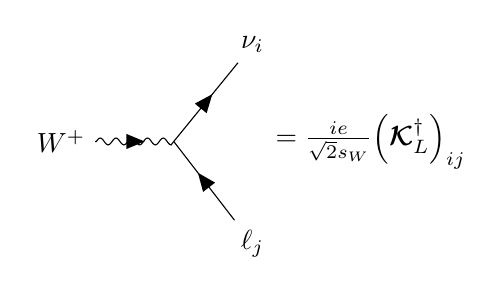
\begin{tikzpicture}
			\begin{feynman}
				\vertex (v1);
				\vertex[right=1cm of v1] (p1);
				\vertex[above=1cm of p1] (o1){\(\nu_{i}\)};
				\vertex[below=1cm of p1] (o2){\(\ell_{j}\)};
				\vertex[left=1cm of v1] (i1) {\(W^{+}\)};
				\diagram*{
				(i1) -- [charged boson] (v1),
				(v1) -- [fermion] (o1),
				(o2) -- [fermion] (v1),
				};
			\end{feynman}
			\node at (2.5,0) {\(=\frac{ie}{\sqrt{2}\sw}\qty(\bm{\cK}^{\dagger}_{L})_{ij}\)};
		\end{tikzpicture}
	\end{subfigure}
	\begin{subfigure}[b]{0.45\linewidth}
		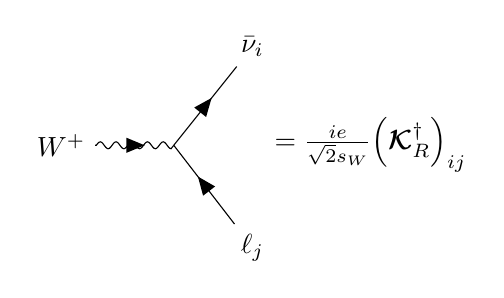
\begin{tikzpicture}
			\begin{feynman}
				\vertex (v1);
				\vertex[right=1cm of v1] (p1);
				\vertex[above=1cm of p1] (o1){\(\rhn_{i}\)};
				\vertex[below=1cm of p1] (o2){\(\ell_{j}\)};
				\vertex[left=1cm of v1] (i1) {\(W^{+}\)};
				\diagram*{
				(i1) -- [charged boson] (v1),
				(v1) -- [fermion] (o1),
				(o2) -- [fermion] (v1),
				};
			\end{feynman}
			\node at (2.5,0) {\(=\frac{ie}{\sqrt{2}\sw}\qty(\bm{\cK}^{\dagger}_{R})_{ij}\)};
		\end{tikzpicture}
	\end{subfigure}\label{fig:feynrules_w_nu}
	\caption{Feynman rules containing a \(W\)-boson, left-handed charged lepton and neutrino.}
\end{figure}


\begin{figure}
	\centering
	\begin{subfigure}[b]{0.45\linewidth}
		\begin{tikzpicture}
			\begin{feynman}
				\vertex (v1);
				\vertex[right=1cm of v1] (p1);
				\vertex[above=1cm of p1] (o1){\(\nu_{i}\)};
				\vertex[below=1cm of p1] (o2){\(\nu_{j}\)};
				\vertex[left=1cm of v1] (i1) {\(Z\)};
				\diagram*{
				(i1) -- [boson] (v1),
				(v1) -- [fermion] (o1),
				(o2) -- [fermion] (v1),
				};
			\end{feynman}
			\node at (3,0) {\(=\frac{ie}{2\cw\sw}\qty(\bm{\cK}_{L}^{\dagger}\bm{\cK}_{L})_{ij}\)};
		\end{tikzpicture}
	\end{subfigure}
	\begin{subfigure}[b]{0.45\linewidth}
		\begin{tikzpicture}
			\begin{feynman}
				\vertex (v1);
				\vertex[right=1cm of v1] (p1);
				\vertex[above=1cm of p1] (o1){\(\nu_{i}\)};
				\vertex[below=1cm of p1] (o2){\(\rhn_{j}\)};
				\vertex[left=1cm of v1] (i1) {\(Z\)};
				\diagram*{
				(i1) -- [boson] (v1),
				(v1) -- [fermion] (o1),
				(o2) -- [fermion] (v1),
				};
			\end{feynman}
			\node at (3,0) {\(=\frac{ie}{2\cw\sw}\qty(\bm{\cK}_{L}^{\dagger}\bm{\cK}_{R})_{ij}\)};
		\end{tikzpicture}
	\end{subfigure}
	\begin{subfigure}[b]{0.45\linewidth}
		\begin{tikzpicture}
			\begin{feynman}
				\vertex (v1);
				\vertex[right=1cm of v1] (p1);
				\vertex[above=1cm of p1] (o1){\(\rhn_{i}\)};
				\vertex[below=1cm of p1] (o2){\(\nu_{j}\)};
				\vertex[left=1cm of v1] (i1) {\(Z\)};
				\diagram*{
				(i1) -- [boson] (v1),
				(v1) -- [fermion] (o1),
				(o2) -- [fermion] (v1),
				};
			\end{feynman}
			\node at (3,0) {\(=\frac{ie}{2\cw\sw}\qty(\bm{\cK}_{R}^{\dagger}\bm{\cK}_{L})_{ij}\)};
		\end{tikzpicture}
	\end{subfigure}
	\begin{subfigure}[b]{0.45\linewidth}
		\begin{tikzpicture}
			\begin{feynman}
				\vertex (v1);
				\vertex[right=1cm of v1] (p1);
				\vertex[above=1cm of p1] (o1){\(\rhn_{i}\)};
				\vertex[below=1cm of p1] (o2){\(\rhn_{j}\)};
				\vertex[left=1cm of v1] (i1) {\(Z\)};
				\diagram*{
				(i1) -- [boson] (v1),
				(v1) -- [fermion] (o1),
				(o2) -- [fermion] (v1),
				};
			\end{feynman}
			\node at (3,0) {\(=\frac{ie}{2\cw\sw}\qty(\bm{\cK}_{R}^{\dagger}\bm{\cK}_{R})_{ij}\)};
		\end{tikzpicture}
	\end{subfigure}\label{fig:feynrules_z_nu}
	\caption{Feynman rules containing a \(Z\)-boson and two neutrinos.}
\end{figure}

\begin{figure}
	\centering
	\begin{subfigure}[b]{0.45\linewidth}
		\begin{tikzpicture}
			\begin{feynman}
				\vertex (v1);
				\vertex[right=1cm of v1] (p1);
				\vertex[above=1cm of p1] (o1){\(\nu_{i}\)};
				\vertex[below=1cm of p1] (o2){\(\ell_{j}\)};
				\vertex[left=1cm of v1] (i1) {\(G^{-}\)};
				\diagram*{
				(i1) -- [anti charged scalar] (v1),
				(v1) -- [fermion] (o1),
				(v1) -- [fermion] (o2),
				};
			\end{feynman}
			\node at (2.5,0) {\(=\frac{\sqrt{2}i}{v}m_{\nu_{i}}\qty(\bm{\cK}_{L}^{\dagger})_{ij}\)};
		\end{tikzpicture}
	\end{subfigure}
	\begin{subfigure}[b]{0.45\linewidth}
		\begin{tikzpicture}
			\begin{feynman}
				\vertex (v1);
				\vertex[right=1cm of v1] (p1);
				\vertex[above=1cm of p1] (o1){\(\rhn_{i}\)};
				\vertex[below=1cm of p1] (o2){\(\ell_{j}\)};
				\vertex[left=1cm of v1] (i1) {\(G^{-}\)};
				\diagram*{
				(i1) -- [anti charged scalar] (v1),
				(v1) -- [fermion] (o1),
				(v1) -- [fermion] (o2),
				};
			\end{feynman}
			\node at (2.5,0) {\(=\frac{\sqrt{2}i}{v}m_{\rhn_{i}}\qty(\bm{\cK}_{R}^{\dagger})_{ij}\)};
		\end{tikzpicture}
	\end{subfigure}
	\begin{subfigure}[b]{0.45\linewidth}
		\begin{tikzpicture}
			\begin{feynman}
				\vertex (v1);
				\vertex[right=1cm of v1] (p1);
				\vertex[above=1cm of p1] (o1){\(\ell_{i}\)};
				\vertex[below=1cm of p1] (o2){\(\nu_{j}\)};
				\vertex[left=1cm of v1] (i1) {\(G^{+}\)};
				\diagram*{
				(i1) -- [charged scalar] (v1),
				(o1) -- [fermion] (v1),
				(o2) -- [fermion] (v1),
				};
			\end{feynman}
			\node at (2.5,0) {\(=\frac{\sqrt{2}i}{v}m_{\nu_{j}}\qty(\bm{\cK}_{L})_{ij}\)};
		\end{tikzpicture}
	\end{subfigure}
	\begin{subfigure}[b]{0.45\linewidth}
		\begin{tikzpicture}
			\begin{feynman}
				\vertex (v1);
				\vertex[right=1cm of v1] (p1);
				\vertex[above=1cm of p1] (o1){\(\ell_{i}\)};
				\vertex[below=1cm of p1] (o2){\(\rhn_{j}\)};
				\vertex[left=1cm of v1] (i1) {\(G^{+}\)};
				\diagram*{
				(i1) -- [charged scalar] (v1),
				(o1) -- [fermion] (v1),
				(o2) -- [fermion] (v1),
				};
			\end{feynman}
			\node at (2.5,0) {\(=\frac{\sqrt{2}i}{v}m_{\rhn_{j}}\qty(\bm{\cK}_{R})_{ij}\)};
		\end{tikzpicture}
	\end{subfigure}
	\label{fig:feynrules_gvl}
	\caption{Feynman rules containing a charged Golstone, a left-handed charged lepton and neutrino.}
\end{figure}

\input{files/appendix/general_rhn/feynman_rules/g_lr_v.tex}
\begin{figure}
	\centering
	\begin{subfigure}[b]{0.5\linewidth}
		\begin{tikzpicture}
			\begin{feynman}
				\vertex (v1);
				\vertex[right=1cm of v1] (p1);
				\vertex[above=1cm of p1] (o1){\(\nu_{i}\)};
				\vertex[below=1cm of p1] (o2){\(\nu_{j}\)};
				\vertex[left=1cm of v1] (i1) {\(h\)};
				\diagram*{
				(i1) -- [scalar] (v1),
				(v1) -- [fermion] (o1),
				(v1) -- [fermion] (o2),
				};
			\end{feynman}
			\node at (4,0) {\(=-\frac{i}{v}\qty(m_{\nu_{i}}\bm{\cK}_{L}^{\dagger}\bm{\cK}_{L} + m_{\nu_{j}}\bm{\cK}_{L}^{T}\bm{\cK}^{*}_{L})_{ij}\)};
		\end{tikzpicture}
	\end{subfigure}
	\begin{subfigure}[b]{0.5\linewidth}
		\begin{tikzpicture}
			\begin{feynman}
				\vertex (v1);
				\vertex[right=1cm of v1] (p1);
				\vertex[above=1cm of p1] (o1){\(\rhn_{i}\)};
				\vertex[below=1cm of p1] (o2){\(\rhn_{j}\)};
				\vertex[left=1cm of v1] (i1) {\(h\)};
				\diagram*{
				(i1) -- [scalar] (v1),
				(v1) -- [fermion] (o1),
				(v1) -- [fermion] (o2),
				};
			\end{feynman}
			\node at (4,0) {\(=-\frac{i}{v}\qty(m_{\rhn_{i}}\bm{\cK}_{R}^{\dagger}\bm{\cK}_{R} + m_{\rhn_{j}}\bm{\cK}_{R}^{T}\bm{\cK}^{*}_{R})_{ij}\)};
		\end{tikzpicture}
	\end{subfigure}
	\begin{subfigure}[b]{0.5\linewidth}
		\begin{tikzpicture}
			\begin{feynman}
				\vertex (v1);
				\vertex[right=1cm of v1] (p1);
				\vertex[above=1cm of p1] (o1){\(\rhn_{i}\)};
				\vertex[below=1cm of p1] (o2){\(\nu_{j}\)};
				\vertex[left=1cm of v1] (i1) {\(h\)};
				\diagram*{
				(i1) -- [scalar] (v1),
				(v1) -- [fermion] (o1),
				(v1) -- [fermion] (o2),
				};
			\end{feynman}
			\node at (4,0) {\(=-\frac{i}{v}\qty(m_{\rhn_{i}}\bm{\cK}_{R}^{T}\bm{\cK}^{*}_{L} + m_{\nu_{j}}\bm{\cK}_{R}^{\dagger}\bm{\cK}_{L})_{ij}\)};
		\end{tikzpicture}
	\end{subfigure}
	\label{fig:feynrules_hvv}
	\caption{Feynman rules containing a Higgs and two neutrinos. The Feynman rules for the
		reversed fermion lines are the conjugate of the ones shown.}
\end{figure}

\input{files/appendix/general_rhn/feynman_rules/g_v_v.tex}


\subsection{Single RH Neutrino}

Here we specialize the above discussion to the case with a single RH neutrino (i.e
\(n=1\)). In this case, the neutrino mass matrix takes the form
\begin{align}
	\hat{\bm{M}} = \mqty(
	0             & 0               & 0                & \hat{m}_{D,e}    \\
	0             & 0               & 0                & \hat{m}_{D,\mu}  \\
	0             & 0               & 0                & \hat{m}_{D,\tau} \\
	\hat{m}_{D,e} & \hat{m}_{D,\mu} & \hat{m}_{D,\tau} & \mu              \\
	)
\end{align}
where \(\hat{m}_{D,\ell} = v y_{\ell}/\sqrt{2}\). For now, we assume the \(\hat{m}_{D,\ell}\)
are real (we relax this later.) The eigenvalues of
\(\hat{\bm{M}}\) are:
\begin{align}
	m_{1} & = m_{2} = 0                                     \\
	m_{3} & = \frac{\mu}{2}\qty(\sqrt{1 + 2\epsilon^{2}}-1) \\
	m_{4} & = \frac{\mu}{2}\qty(\sqrt{1 + 2\epsilon^{2}}+1)
\end{align}
where \(\epsilon=vy/\mu\) and \(y^{2}=y_{e}^{2}+y_{\mu}^{2}+y_{\tau}^{2}\).
Then mass eigenstates are:
\begin{align}
	\nu_{1} & = \frac{1}{\sqrt{y^{2}_{e}\qty(y^{2}_{\mu} + y^{2}_{\tau})}}
	\mqty(0                                                                               \\
	-y_{e}y_{\tau}                                                                        \\
	y_{e}y_{\mu}                                                                          \\
	0),     &
	\nu_{2} & = \frac{1}{\sqrt{y^{2}y_{\tau}^2y_{\mu}^{2}\qty(y_{\mu}^{2}+y_{\tau}^{2})}}
	\mqty(
	-y_{\mu}y_{\tau}\qty(y_{\mu}^{2}+y_{\tau}^{2})                                        \\
	y_{e}y^{2}_{\mu}y_{\tau}                                                              \\
	y_{e}y_{\mu}y^{2}_{\tau}                                                              \\
	0)                                                                                    \\
	\nu_{3} & = \frac{i}{\sqrt{2m^{2}_{3} + v^2y^2}}
	\mqty(
	v y_{e}                                                                               \\
	v y_{\mu}                                                                             \\
	v y_{\tau}                                                                            \\
	-\sqrt{2}m_{3}
	),      &
	\nu_{4} & = \frac{1}{\sqrt{2m^{2}_{4} + v^2y^2}}
	\mqty(
	v y_{e}                                                                               \\
	v y_{\mu}                                                                             \\
	v y_{\tau}                                                                            \\
	-\sqrt{2}m_{4}
	)
\end{align}
with \(\Omega\) being the matrix with the eigenstates as columns. If we set
\(y_{\tau} = y\) and \(y_{e}=y_{\mu}=0\), we \(\Omega\) is (which we will denote
as \(\Omega_{0}\))
\begin{align}
	\Omega_{0}
	  & =
	\mqty(
	1 & 0 & 0                            & 0                           \\
	0 & 1 & 0                            & 0                           \\
	0 & 0 & i\sqrt{\frac{m_4}{m_4+m_3}}  & \sqrt{\frac{m_3}{m_4+m_3}}  \\
	0 & 0 & -i\sqrt{\frac{m_3}{m_4+m_3}} & \sqrt{\frac{m_4}{m_4+m_3}})
\end{align}
If we define a mixing angle \(\theta\) such that:
\begin{align}
	\cos\theta & = \sqrt{\frac{m_4}{m_4+m_3}}, &
	\sin\theta & = \sqrt{\frac{m_3}{m_4+m_3}}
\end{align}
then \(\tan^2\theta = m_{3}/m_{4}\). We can therefore define all the parameters in
terms of the mixing angle and the heavy mass. Let \(m_{\nu}=m_{3}\) and
\(m_{4} = m_{\rhn}\). Then,
\begin{align}
	m_{\nu} & = m_{\rhn}\tan^2\theta,                 &
	y       & = \frac{\sqrt{2}m_{\rhn}}{v}\tan\theta, &
	\mu     & = m_{\rhn}\qty(1-\tan^2\theta)
\end{align}
In the case where \(y_{e},y_{\mu}\) and \(y_{\tau}\) are all non-zero, then we
first perform a rotation such that we remove \(y_{e}\) and \(y_{\mu}\). This is
done using a rotation matrix \(R\) such that:
\begin{align}
	R^{T}\hat{\bm{M}}R =
	\mqty(
	0 & 0 & 0                  & 0                  \\
	0 & 0 & 0                  & 0                  \\
	0 & 0 & 0                  & \sqrt{v}y/\sqrt{2} \\
	0 & 0 & \sqrt{v}y/\sqrt{2} & \mu                \\
	)
\end{align}
To achive this, we use the following rotation matrix:
\begin{align}
	R = \mqty(
	\cos\alpha\cos\beta & -\sin\beta & \cos\beta\sin\alpha & 0 \\
	\cos\alpha\sin\beta & \cos\beta  & \sin\alpha\sin\beta & 0 \\
	-\sin\alpha         & 0          & \cos\alpha          & 0 \\
	0                   & 0          & 0                   & 1
	)
\end{align}
where \(\alpha\) and \(\beta\) are such that
\begin{align}
	y_{e}    & = y\cos\beta\sin\alpha, &
	y_{\mu}  & = y\sin\beta\sin\alpha, &
	y_{\tau} & = y\cos\alpha,          &
\end{align}
Then, \(R^{T}\hat{\bm{M}}R\) is diagonalized using the above \(\Omega_{0}\). That
is, \(\Omega^{T}_{0}R^{T}\hat{\bm{M}}R\Omega_{0}\) is diagonal. And therefore, we
identify the full roation matrix as \(\Omega = R\Omega_{0}\), which is:
\begin{align}
	\Omega = \mqty(
	\cos\alpha\cos\beta & -\sin\beta & i \sin\alpha\cos\beta\cos\theta & \sin\alpha\cos\beta\sin\theta \\
	\cos\alpha\sin\beta & \cos\beta  & i \sin\alpha\sin\beta\cos\theta & \sin\alpha\sin\beta\sin\theta \\
	-\sin\alpha         & 0          & i \cos\alpha\cos\theta          & \cos\alpha\sin\theta          \\
	0                   & 0          & -i \sin\theta                   & \cos\theta                    \\
	)
\end{align}

Lastly, we let the \(y_{\ell}\) be complex. In this case, we need to remove the
phases before applying the above \(\Omega\). We can write
\(\tilde{y}_{\ell}= y_{\ell}e^{i\delta_{\ell}}\). We can rephase the RH-Neutrino field
to absorb the phase of \(\mu\). Thus, the mass matrix with complex Yukawas is:
\begin{align}
	\hat{\bm{M}} = \frac{v}{\sqrt{2}}\mqty(
	0             & 0               & 0                & \tilde{y}_{e}    \\
	0             & 0               & 0                & \tilde{y}_{\mu}  \\
	0             & 0               & 0                & \tilde{y}_{\tau} \\
	\tilde{y}_{e} & \tilde{y}_{\mu} & \tilde{y}_{\tau} & \sqrt{2}\mu/v    \\
	)
\end{align}
Applying a phase matrix \(\bm{P}\) to the mass matrix as \(\bm{P}^{T}\hat{\bm{M}}\bm{P}\)
removes all of the phases. Here, the matrix \(\bm{P}\) is given by:
\begin{align}
	\bm{P}
	=
	\mqty(\dmat{
		e^{-i\delta_{e}} ,
		e^{-i\delta_{\mu}},
		e^{-i\delta_{\tau}},
		1
	})
\end{align}
Thus, the full mixing matrix \(\Omega\) for the neutrinos is given by the following product of
rotations and phases:
\begin{align}
	\Omega      & =
	\mqty(\dmat{
		e^{-i\delta_{e}} ,
		e^{-i\delta_{\mu}},
		e^{-i\delta_{\tau}},
		1
	})
	\mqty(
	\dmat{
	\cos\beta   & -\sin\beta                   \\
	\sin\beta   & \cos\beta,1,1}
	)                                          \\
	            & \quad\times
	\mqty(\dmat{
	\cos\alpha  &                & \sin\alpha  \\
	            & 1              &             \\
	-\sin\alpha &                & \cos\alpha,
		1
	})
	\mqty(\dmat{
		1,1,
	\cos\theta  & \sin\theta                   \\
	-\sin\theta & \cos\theta                   \\
	})
	\mqty(\dmat{1,1,e^{i\pi/2},1})
\end{align}
If we take the 3 angles and the heavy neutrino mass as our parameters, the
yukawas and majorana mass are given by:
\begin{align}
	\tilde{y}_{e}    & =\frac{\sqrt{2}m_{\rhn}}{v}\tan\theta\cos\beta\sin\alpha e^{i\delta_{e}},   &
	\tilde{y}_{\mu}  & =\frac{\sqrt{2}m_{\rhn}}{v}\tan\theta\sin\beta\sin\alpha e^{i\delta_{\mu}},   \\
	\tilde{y}_{\tau} & =\frac{\sqrt{2}m_{\rhn}}{v}\tan\theta\cos\alpha e^{i\delta_{\tau}},         &
	\mu              & = m_{\rhn}(1-\tan^2\theta)
\end{align}
and the light neutrino mass is \(m_{\nu} = m_{\rhn}\tan^2\theta\). Additionally, the
PMNS matrices are:
\begin{align}
	\bm{\cK}_{L}
	                                      &
	=
	\mqty(
	e^{-i\delta_{e}}\cos\alpha\cos\beta   &
	-e^{-i\delta_{e}}\sin\beta            &
	i \sin\alpha\cos\beta\cos\theta                   \\
	%e^{-i\delta_{e}}\sin\alpha\cos\beta\sin\theta                             \\
	%----
	e^{-i\delta_{\mu}}\cos\alpha\sin\beta &
	e^{-i\delta_{\mu}}\cos\beta           &
	i e^{-i\delta_{\mu}}\sin\alpha\sin\beta\cos\theta \\
	%& e^{-i\delta_{\mu}}\sin\alpha\sin\beta\sin\theta \\
	%----
	-e^{-i\delta_{\tau}}\sin\alpha        &
	0                                     &
	i e^{-i\delta_{\tau}}\cos\alpha\cos\theta
	%& \cos\alpha\sin\theta          \\
	)                                                 \\
	\bm{\cK}_{R}
	                                      &
	=
	\mqty(
	%e^{-i\delta_{e}}\cos\alpha\cos\beta   &
	%-e^{-i\delta_{e}}\sin\beta            &
	%i \sin\alpha\cos\beta\cos\theta                   \\
	e^{-i\delta_{e}}\sin\alpha\cos\beta\sin\theta     \\
	%----
	%e^{-i\delta_{\mu}}\cos\alpha\sin\beta &
	%e^{-i\delta_{\mu}}\cos\beta           &
	%i e^{-i\delta_{\mu}}\sin\alpha\sin\beta\cos\theta \\
	e^{-i\delta_{\mu}}\sin\alpha\sin\beta\sin\theta   \\
	%----
	%-e^{-i\delta_{\tau}}\sin\alpha        &
	%0                                     &
	%i e^{-i\delta_{\tau}}\cos\alpha\cos\theta
	\cos\alpha\sin\theta                              \\
	)
\end{align}




In the above parameterization, we can see that cases of the RH-neutrino mixing with only
a single LH-neutrino are:
\begin{align}
	\text{electron} & : & \beta & =0,                 & \alpha & =\pi/2, \\
	\text{muon}     & : & \beta & =\pi/2,             & \alpha & =\pi/2, \\
	\text{tau}      & : & \beta & =\mathrm{anything}, & \alpha & =0
\end{align}





\section{Matching Onto Chiral Lagrangian}

In this appendix, we show how to match the RH neutrino Lagragian onto the chiral
Lagragian to obtain interactions containings the RH neutrino and mesons.

\subsection{Leading Order Chiral Lagrangian}

Recall that the leading-order chiral Lagrangian is given by:
\begin{align}
    \cL_{\ChiPT} & = \frac{f_{\pi}^{2}}{4}\Tr[
        \qty(D_{\mu}\bm{\Sigma})^{\dagger}
        \qty(D^{\mu}\bm{\Sigma})
    ]
    + \frac{f_{\pi}^{2}}{4}\Tr[\bm{\chi}\bm{\Sigma}^{\dagger} + \mathrm{c.c.}]
\end{align}
where \(f_{\pi}\) is the pion decay constant, \(\bm{\Sigma}\) is the Goldstone
matrix \(\exp(i\frac{i}{f_{\pi}}\phi_{a}\bm{\lambda}_{a})\),
\(D_{\mu}\) is the chiral covariant derivative, and
\(\bm{\chi} = 2B_{0}\bm{M}_{q}\). The \(\phi_{a}\) fields are such that
\begin{align}
    \phi_{a}\bm{\lambda}_{a} =
    \mqty(
    \pi^{0} + \eta/\sqrt{3} & \sqrt{2}\pi^{+}         & \sqrt{2}k^{+}           \\
    \sqrt{2}\pi^{-}         & -\pi^{0} +\eta/\sqrt{3} & \sqrt{2}k^{0}           \\
    \sqrt{2}k^{-}           & \sqrt{2}\bar{k}^{0}     & -\sqrt{\frac{2}{3}}\eta \\
    )
\end{align}
with \(\bm{\lambda}_{a}\) being the Gell-Mann matrices. The chiral covariant
derivative is given by:
\begin{align}
    D_{\mu}\bm{\Sigma} = \partial_{\mu}\bm{\Sigma} - i\bm{R}_{\mu}\bm{\Sigma} + i\bm{\Sigma}\bm{L}_{\mu}
\end{align}
with \(\bm{R}_{\mu}\) and \(\bm{L}_{\mu}\) the right and left handed quark currents.
The Goldstone matrix can be expanded in terms of the \(\phi\) fields and the Gell-Mann
matrices. If we write \(\bm{\Sigma} = \Sigma_{0}\bm{I} + \Sigma_{a}\bm{\lambda}_{a}\),
then:
\begin{align}
    \Sigma_{0}
     & =
    1
    + \frac{2}{3}S_{2}\expval{\phi^2}
    + \frac{2}{3}S_{3}\expval{\phi^3 d}
    + \frac{2}{3}S_{4}\expval{\phi^2}^{2}
    + \cdots \\
    \Sigma_{a}
     & =
    S_{1}\phi_{k}
    + S_{2}\expval{\phi^{2}d}_{k}
    + S_{3}\expval{\phi^{2}} \phi_{k}
    + S_{4}\qty(\frac{2}{3}\expval{\phi^{3}d}\phi_{k} + \expval{\phi}^{2}\expval{\phi^{2}d}_{k})
    + \cdots
\end{align}
where \(S_{n} = \frac{1}{n!}\qty(\frac{i}{f_{\pi}})^{n}\) and
\begin{align}
    \expval{\phi^{2}}
     & \equiv
    \phi_{a}\phi_{a},
     &
    \expval{\phi^{2}d}_{k}
     & \equiv
    \phi_{a}\phi_{b}d^{abk},
     &
    \expval{\phi^{3}d}
     & \equiv
    \phi_{a}\phi_{b}\phi_{c}d^{abc}
\end{align}
with \(d^{abc} = \frac{1}{4}\Tr[\bm{\lambda}_{a}\acomm{\bm{\lambda}_{b}}{\bm{\lambda}_{c}}]\).
The chiral kinetic term can be written as
\begin{align}
    \Tr[
        \qty(D_{\mu}\bm{\Sigma})^{\dagger}
        \qty(D^{\mu}\bm{\Sigma})
    ] = T_{2} + T_{3} + T_{4}
\end{align}
where
\begin{align}
    T_{2} & = \Tr[
        \qty(\partial_{\mu}\bm{\Sigma})^{\dagger}
        \qty(\partial_{\mu}\bm{\Sigma})
        + \bm{R}^{\dagger}_{\mu}\bm{R}_{\mu}
        + \bm{L}^{\dagger}_{\mu}\bm{L}_{\mu}
    ]               \\
    T_{3} & = i\Tr[
        \qty(\partial_{\mu}\bm{\Sigma})^{\dagger}
        \qty(
        \bm{\Sigma}\bm{L}_{\mu} -
        \bm{R}_{\mu}\bm{\Sigma}
        ) + \mathrm{c.c.}
    ]               \\
    T_{4} & = -\Tr[
        \bm{\Sigma}
        \bm{L}_{\mu}
        \bm{\Sigma}^{\dagger}
        \bm{R}^{\dagger}_{\mu}
    ]-\Tr[
        \bm{R}_{\mu}
        \bm{\Sigma}
        \bm{L}^{\dagger}_{\mu}
        \bm{\Sigma}^{\dagger}
    ]
\end{align}
If we define
\(\bm{L}_{\mu} = L_{\mu}^{0}\bm{I} + L^{a}_{\mu}\bm{\lambda}_{a}\) and
\(\bm{R}_{\mu} = R_{\mu}^{0}\bm{I} + R^{a}_{\mu}\bm{\lambda}_{a}\), then
\(T_{2}\) is
\begin{align}
    T_{2} & =
    3\qty(\qty|\partial_{\mu}\Sigma_{0}|^{2} + \qty|R^{0}_{\mu}|^{2} + \qty|L^{0}_{\mu}|^{2})
    +
    2\qty(\qty|\partial_{\mu}\Sigma_{a}|^{2} + \qty|R^{a}_{\mu}|^{2}+ \qty|L^{a}_{\mu}|^{2})
\end{align}
The second term is given by:
\begin{align}
    T_{3}
     & =
    3i\qty(L^{0}_{\mu}-R^{0}_{\mu})\Sigma_{0}\qty(\partial^{\mu}\Sigma_{0})^{\dagger} \\
     & \quad
    + 2i\qty[
        \qty(L^{a}_{\mu}-R^{a}_{\mu})
        \qty[
            \Sigma^{a}\qty(\partial^{\mu}\Sigma^{0})^{\dagger} +
            \Sigma^{0}\qty(\partial^{\mu}\Sigma^{a})^{\dagger}
        ] +
        \qty(L^{0}_{\mu}-R^{0}_{\mu})\Sigma^{a}\qty(\partial^{\mu}\Sigma^{a})^{\dagger}
    ]\notag                                                                           \\
     & \quad
    +2i\qty[
    \qty(L^{a}_{\mu}-R^{a}_{\mu})\Sigma^{b}\qty(\partial^{\mu}\Sigma^{c})^{\dagger}d_{abc} +
    i\qty(L^{a}_{\mu}+R^{a}_{\mu})\Sigma^{b}\qty(\partial^{\mu}\Sigma^{c})^{\dagger}f_{abc}
    ]\notag                                                                           \\
     & \quad
    + \mathrm{c.c.}\notag
\end{align}
The last term is given by
\begin{align}
    T_{4}
     & =
    \qty(3\qty|\Sigma_0|^{\dagger} + 2\Sigma^{\dagger}_{a}\Sigma_{a})R^{\dagger}_{0}L_{0}
    + 2\qty|\Sigma_{0}|^{2}R^{a}_{\mu}L_{a}               \\
     & \quad +
    2\qty(
    \Sigma_{0}\Sigma^{\dagger}_{a}
    +\Sigma_{a}\Sigma^{\dagger}_{0}
    )
    \qty(R^{a}_{\mu}L_{0} + R^{0}_{\mu}L^{a}_{\mu})\notag \\
     & \quad +
    2\qty[
    \Sigma^{\dagger}_{a}\qty(R^{b}_{\mu})^{\dagger}\Sigma_{c}L^{0}_{\mu} +
    \Sigma^{\dagger}_{a}\qty(R^{0}_{\mu})^{\dagger}\Sigma_{b}L^{c}_{\mu} +
    \Sigma^{\dagger}_{a}\qty(R^{b}_{\mu})^{\dagger}\Sigma_{0}L^{c}_{\mu} +
    \Sigma^{\dagger}_{0}\qty(R^{a}_{\mu})^{\dagger}\Sigma_{b}L^{c}_{\mu}
    ]\qty(d^{abc} + if^{abc})
    \notag                                                \\
     & \quad
    + \frac{4}{3}\Sigma^{\dagger}_{a}\qty(R^{a}_{\mu})^{\dagger}\Sigma_{b}L^{b}_{\mu}
    + 2\Sigma^{\dagger}_{a}\qty(R^{b}_{\mu})^{\dagger}\Sigma_{c}L^{d}_{\mu}
    \qty(d^{abe} +i f^{abe} )
    \qty(d^{cde} +i f^{cde} )\notag                       \\
     & \quad
    +\mathrm{c.c.}
\end{align}

\subsection{Matching Four-Fermi Interactions}
The low energy effective theory of the light SM fields is given by the
four-fermi Lagrangian, obtained by integrating out the \(W^{\pm}\) and
\(Z\). The result of integrating out the heavy bosons is:
\begin{align}
    \cL_{4F} = -\frac{4G_{F}}{\sqrt{2}}\qty[J^{+}_{\mu}J^{-}_{\mu} + \qty(J^{Z}_{\mu})^{2}]
\end{align}
In the above expression, the charged and neutral currents are given by:
\begin{align}
    J^{+}_{\mu}      & = j^{+}_{\mu}
    + V_{ud}u^{\dagger}\bar{\sigma}_{\mu}d
    + V_{us}u^{\dagger}\bar{\sigma}_{\mu}s
    \\
    J^{-}_{\mu}      & = j^{-}_{\mu}
    + V^{*}_{ud}d^{\dagger}\bar{\sigma}_{\mu}u
    + V^{*}_{us}s^{\dagger}\bar{\sigma}_{\mu}u
    \\
    c_{W}J^{Z}_{\mu} & = c_{W}j^{Z}_{\mu} +
    \sum_{q=u,d,s}\qty(g_{L,q}q^{\dagger}\bar{\sigma}_{\mu}q
    +g_{R,q}\bar{q}^{\dagger}\bar{\sigma}_{\mu}\bar{q})
\end{align}
where \(j^{\pm}_{\mu}(j^{Z}_{\mu})\) are the charged(neutral) currents without light quarks,
\(V_{ij}\) is the CKM matrix and left/right handed couplings are
\begin{align}
    g_{L,u} & = \frac{1}{2} - \frac{2}{3}s_{W}^{2}  &
    g_{L,d} & = -\frac{1}{2} + \frac{1}{3}s_{W}^{2} &
    g_{R,u} & = -\frac{2}{3}s_{W}^{2}               &
    g_{R,d} & = \frac{1}{3}s_{W}^{2}
\end{align}
In terms of the left-handed neutrino gauge eigenstates, the charged and neutral currents
are given by:
\begin{align}
    j^{Z}_{\mu} & =
    \frac{1}{2c_{W}}\hat{\nu}_{i}^{\dagger}\bar{\sigma}_{\mu}\hat{\nu}_{i}
    +\frac{1}{2c_{W}}\qty(-1+2s_{W}^{2})\ell_{i}^{\dagger}\bar{\sigma}_{\mu}\ell_{i}
    -\frac{s_{W}^{2}}{c_{W}}\bar{\ell}_{i}^{\dagger}\bar{\sigma}_{\mu}\bar{\ell}_{i} \\
    j^{+}_{\mu} & =\hat{\nu}_{i}^{\dagger}\bar{\sigma}_{\mu}\ell_{i}
\end{align}
Grouping the left-handed light quarks into a vector \(\bm{q} = \mqty(u & d & s)\)
and the right-handed quarks into
\(\bar{\bm{q}} = \mqty(\bar{u} & \bar{d} & \bar{s})\), we can write the currents
as
\begin{align}
    J^{+}_{\mu}      & = j^{+}_{\mu}
    +
    \bm{q}^{\dagger}\bm{V}\bar{\sigma}_{\mu}\bm{q}
    \\
    J^{-}_{\mu}      & = j^{-}_{\mu}
    + \bm{q}^{\dagger}\bm{V}^{\dagger}\bar{\sigma}_{\mu}\bm{q}
    \\
    c_{W}J^{Z}_{\mu} & = c_{W}j^{Z}_{\mu} +
    \bm{q}^{\dagger}\bm{G}_{L}\bar{\sigma}_{\mu}\bm{q} +
    \bar{\bm{q}}^{\dagger}\bm{G}_{R}\bar{\sigma}_{\mu}\bar{\bm{q}}
\end{align}
where
\begin{align}
    \bm{V}
            & =
    \mqty(0 & V_{ud} & V_{us} \\ 0&0&0\\ 0&0&0),
            &
    \bm{G}_{L,q}
            & =
    \bm{T}_{3,q} - s_{W}^{2}\bm{Q}_{q},
            &
    \bm{G}_{R,q}
            & =
    -s_{W}^{2}\bm{Q}_{q}
\end{align}
with \(\bm{Q}_{q}\) the light-quark charge matrix and \(\bm{T}_{3,q}\) a matrix
containing the light-quark weak-isospin eigenvalues
\begin{align}
    \bm{Q}_{q}
     & =
    \frac{1}{3}\mqty(\dmat{2,-1,-1}),
     &
    \bm{T}_{3,q}
     & =
    \frac{1}{2}\mqty(\dmat{1,-1,-1}),
\end{align}
Expanding out the four-fermi Lagrangian, one finds:
\begin{align}
    %\bm{q}^{\dagger}\bm{V}\bar{\sigma}_{\mu}\bm{q}
    %\bm{q}^{\dagger}\bm{V}^{\dagger}\bar{\sigma}_{\mu}\bm{q}
    %
    %
    -\frac{\sqrt{2}}{4G_{F}}\cL_{4F}
     & =
    \bm{q}^{\dagger}\qty(
    \bm{V}j^{-}_{\mu}
    + \bm{V}^{\dagger}j^{+}_{\mu}
    + \frac{2}{c_{W}}\bm{G}_{L,q}j^{Z}_{\mu}
    )\bar{\sigma}^{\mu}\bm{q}
    +\frac{2}{c_{W}}
    \bar{\bm{q}}^{\dagger}\qty(
    \bm{G}_{R,q}j^{Z}_{\mu}
    )\bar{\sigma}^{\mu}\bar{\bm{q}} \\
     & \quad
    + j^{+}_{\mu}j^{-}_{\mu}
    + j^{Z}_{\mu}j^{Z}_{\mu}\notag  \\
     & \quad
    \qty(\bm{q}^{\dagger}\bm{V}\bar{\sigma}_{\mu}\bm{q})
    \qty(\bm{q}^{\dagger}\bm{V}^{\dagger}\bar{\sigma}_{\mu}\bm{q})
    + \qty(\bm{q}^{\dagger}\bm{G}_{L}\bar{\sigma}_{\mu}\bm{q} +
    \bar{\bm{q}}^{\dagger}\bm{G}_{R}\bar{\sigma}_{\mu}\bar{\bm{q}})^{2}
    \notag
\end{align}
Only the first four terms in the above expression will result in neutrino
interactions (the last two terms contribute to weak interactions among mesons.)
The first two terms are matched onto the left and right handed chiral currents,
resulting in:
\begin{align}
    \cL_{\ChiPT} & \supset \frac{f_{\pi}^{2}}{4}\Tr[
        \qty(D_{\mu}\bm{\Sigma})^{\dagger}
        \qty(D^{\mu}\bm{\Sigma})
    ]
\end{align}
with
\begin{align}
    D_{\mu}\bm{\Sigma}
     & =
    \partial_{\mu}\bm{\Sigma}
    - i\bm{R}_{\mu}\bm{\Sigma}
    + i\bm{\Sigma}\bm{L}_{\mu}, \\
    \bm{R}_{\mu}
     & =
    \frac{2}{c_{W}}
    \bm{G}_{R,q}j^{Z}_{\mu},
     &
    \bm{L}_{\mu}
     & =
    \bm{V}j^{-}_{\mu}
    + \bm{V}^{\dagger}j^{+}_{\mu}
    + \frac{2}{c_{W}}\bm{G}_{L,q}j^{Z}_{\mu}
\end{align}
Note that we can decompose the currents into Gell-Mann matrices, yielding:
\begin{align}
    \bm{L}_{\mu}
     & =
    -\frac{1}{3c_{W}}j^{Z}_{\mu}\bm{I}
    +\frac{2(1-s_{W}^{2})}{c_{W}}\qty(\bm{\lambda}_{3}+\frac{1}{\sqrt{3}}\bm{\lambda}_{8})j^{Z}_{\mu}
    +
    \qty[
    \qty(
    V^{*}_{ud}\bm{\lambda}^{+}_{12} + V^{*}_{us}\bm{\lambda}^{+}_{45}
    )j^{+}_{\mu}
    +\mathrm{c.c.}
    ]\notag \\
    \bm{R}_{\mu}
     & =
    -\frac{2s_{W}^{2}}{c_{W}^{2}}
    \qty(\bm{\lambda}_{3}+\frac{1}{\sqrt{3}}\bm{\lambda}_{8})j^{Z}_{\mu}
\end{align}
where \(\bm{\lambda}^{\pm}_{12} = \bm{\lambda}_{1} \mp i\bm{\lambda}_{2}\) and
\(\bm{\lambda}^{\pm}_{45} = \bm{\lambda}_{4} \mp i\bm{\lambda}_{5}\).
The Lagrangian containing currents and mesons can be brought into the following
form:
\begin{align}
    \cL & =
    -\frac{4G_{F}}{\sqrt{2}}\qty(
    j^{Z}_{\mu}\cJ^{0}_{\mu}
    + \qty(j^{+}_{\mu}\cJ^{+}_{0} + \mathrm{c.c.})
    +\qty(j^{Z}_{\mu})^{2}\cS^{0}
    +j^{Z}_{\mu}\qty(j^{+}_{\mu}\cS^{+}+\mathrm{c.c.})
    )
\end{align}
Here, the neutral meson current \(\cJ^{0}_{\mu}\) is given by:
\begin{align}
    \cJ^{0}_{\mu} & =
    \frac{f_{\pi}}{c_{W}}\qty[
        \partial^{\mu}\pi^{0}
        + \frac{1}{\sqrt{3}}
        \partial^{\mu}\eta
    ]
    - \frac{i (1-2s_{W}^{2})}{c_{W}}
    \qty[
    \pi^{+}\overleftrightarrow{\partial}_{\mu}\pi^{-} +
    K^{+}\overleftrightarrow{\partial}_{\mu}K^{-}
    ]
\end{align}
where \(X\overleftrightarrow{\partial}_{\mu}Y \equiv X\partial_{\mu}Y - Y\partial_{\mu}X\).
The charged meson current is:
\begin{align}
    \cJ^{+}_{\mu}
     & =
    \frac{f_{\pi}}{\sqrt{2}}\qty[
    V^{*}_{ud}\partial^{\mu}\pi^{+}
    + V^{*}_{us}\partial^{\mu}K^{+}
    ]
    \\
     & \quad
    + i
    \frac{V^{*}_{ud}}{\sqrt{2}}\qty(
    \bar{K}^{0}\overleftrightarrow{\partial}_{\mu}K^{+}
    + \sqrt{2}\pi^{+}\overleftrightarrow{\partial}_{\mu}\pi^{0}
    )\notag  \\
     & \quad
    +i\frac{V_{us}^{*}}{2}\qty(
    K^{0}\overleftrightarrow{\partial}_{\mu}\pi^{+}
    +\sqrt{\frac{3}{2}}K^{+}\overleftrightarrow{\partial}_{\mu}\eta
    +\frac{1}{\sqrt{2}}K^{+}\overleftrightarrow{\partial}_{\mu}\pi^{0}
    )\notag
\end{align}
The neutral meson density \(\cS_{0}\) is
\begin{align}
    \cS^{0} & =
    - \frac{4(1-s_{W}^{2})s_{W}^{2}}{c_{W}^{2}}
    \qty[
    \pi^{+}\pi^{-} +
    K^{+}K^{-}
    ]
\end{align}
and the charged meson density \(\cS_{+}\) is
\begin{align}
    \cS^{+} & =
    \frac{s_{W}^{2}}{c_{W}}\qty(
    V^{*}_{ud}\qty(
    \sqrt{2}\pi^{+}\pi^{0}
    - K^{+}\bar{K}^{0}
    )
    +V^{*}_{us}\qty(
    \sqrt{\frac{3}{2}}K^{+}\eta
    + \frac{1}{\sqrt{2}}K^{+}\pi^{0}
    - \pi^{+}K^{0}
    )
    )
\end{align}

\section{Right-Handed Neutrino Partial Widths}

\subsection{Two-Body Partial Widths}
Here we compute the partial widths of the general RH neutrino model. First, we
compute the widths for right-handed neutrinos, decaying into a Higgs, Z-boson and
W-boson. We will then compute the widths into meson final states.

\subsubsection{\texorpdfstring{\(\rhn_{i}\to\nu_{j}h\)}{RH-Neutrino to LH-Neutrino and Higgs}}
The amplitude for \(\rhn_{i}(P) \to H(p_{h}) + \nu_j(p_{\nu})\) is given by:
\begin{align}
	\cM & = 2i \qty[G_{ij}y(p_{\nu})x(P) + G^{*}_{ij}x^{\dagger}(p_{\nu})y^{\dagger}(P)]
\end{align}
where \(G_{ij} = \qty(\bm{\cK}_{L}^{\dagger}\bm{\cK}_{R})_{ij}\). Squaring an summing
over spins, we find:
\begin{align}
	\frac{1}{2}\sum_{\mathrm{spins}}\qty|\cM|^2
	 & =
	4\qty[\qty(m_{\rhn}^2+m_{\nu_{j}}^2 - m_{h}^2) \qty|G_{ij}|^2 + 2m_{\rhn_{i}}m_{\nu_{j}}\Re(G_{ij}^2)]
\end{align}
The partial width is therefore:
\begin{align}
	\Gamma(\rhn_{i}\to \nu_{j}h)
	 & =
	\frac{\lambda^{1/2}(m^{2}_{\rhn_{i}},m_{\nu_{j}}^2,m_{h}^{2})}{16\pi v^{2}m^{3}_{\rhn^{2}_{i}}}
	\bigg{[}
	\qty(m_{\rhn_{i}}^4+m_{\nu_{j}}^4 - m_{h}^2\qty(m_{\rhn_{i}}^2+m_{\nu_{j}}^2) + 6m_{\rhn_{i}}^2m_{\nu_{j}}^2) \qty|G_{ij}|^2 \\
	 & \quad\quad + 2m_{\nu_{j}}m_{\rhn_{i}}\qty(2m_{\rhn_{i}}^2 + 2m_{\nu_{j}}^2 - m_{h}^2)\Re(G_{ij}^2)
	\bigg{]}\notag                                                                                                               \\
	 & \quad\times \theta(m_{\rhn_{i}}-m_{\nu_{j}}-m_{h})\notag
\end{align}

\subsubsection{\texorpdfstring{\(\rhn_{i}\to\nu_{j}Z\)}{RH-Neutrino to LH-Neutrino and Z-Boson}}
The amplitude for \(\rhn_{i}(P) \to Z(p_{Z}) + \nu_j(p_{\nu})\) is given by:
\begin{align}
    \cM & = -iG_{ij} \frac{e}{c_{W}s_{W}}\qty[x^{\dagger}(p_{\nu})\bar{\sigma}_{\mu}x(P)
        - y^{\dagger}(P)\bar{\sigma}_{\mu}y(p_{\nu})]\epsilon^{*}_{\mu}
\end{align}
where \(G_{ij} = \qty(\OmegaVVb^{\dagger}\OmegaVNb)_{ij}\). Squaring and summing
over spins, we find:
\begin{align}
    \frac{1}{2}\sum_{\mathrm{spins}}\qty|\cM|^2
     & =
    \frac{e^{2}\qty|G_{ij}|^2}{s^{2}_{W}M_{W}^{2}}
    \qty(\qty(m_{\rhn_{i}}+m_{\nu_{i}})^{2}-M_{Z}^{2})
    \qty(\qty(m_{\rhn_{i}}-m_{\nu_{i}})^{2}+2M_{Z}^{2})
\end{align}
The partial width is therefore:
% prefactor \lambda^{1/2}(m^{2}_{\rhn_{i}},m_{1}^2,m_{2}^{2}) / (16\pi m^{3}_{\rhn^{2}_{i}})
\begin{align}
    \Gamma(\rhn_{i}\to \nu_{j}Z)
     & =
    \frac{e^{2}\lambda^{1/2}(m^{2}_{\rhn_{i}},m_{\nu_{j}}^2,M_{Z}^{2})}{16\pi s^{2}_{W}M^{2}_{W}m^{3}_{\rhn^{2}_{i}}}
    \qty|\qty(\OmegaVVb^{\dagger}\OmegaVNb)_{ij}|^2
    \qty(\qty(m_{\rhn_{i}}+m_{\nu_{i}})^{2}-M_{Z}^{2})\notag          \\
     & \quad\times\qty(\qty(m_{\rhn_{i}}-m_{\nu_{i}})^{2}+2M_{Z}^{2})
    \theta(m_{\rhn_{i}}-m_{\nu_{j}}-M_{Z})
\end{align}

\subsubsection{\texorpdfstring{\(\rhn_{i}\to\ell_{j}W^{+}\)}{RH-Neutrino to Charged-Lepton and W-Boson}}
The amplitude for \(\rhn_{i}(P) \to W^{+}(p_{W}) + \ell_{j}(p_{\ell})\) is given by:
\begin{align}
    \cM & = -i\frac{e}{\sqrt{2}s_{W}}G_{ij} x^{\dagger}(p_{\ell})\bar{\sigma}_{\mu}x(P)
\end{align}
where \(G_{ij} = \qty(\OmegaVNb)_{ij}\). Squaring and summing
over spins, we find:
\begin{align}
    \frac{1}{2}\sum_{\mathrm{spins}}\qty|\cM|^2
     & =
    \frac{e^{2}\qty|\OmegaVNb^{ij}|^2}{4M_{W}^{2}}
    \qty(
    \qty(m_{\rhn_{i}}-m_{\ell_{j}})^{2}
    +\qty(m^{2}_{\rhn_{i}}+m^{2}_{\ell_{j}})M_{W}^{2}
    -2M_{W}^{4}
    )
\end{align}
The partial width is therefore:
% prefactor \lambda^{1/2}(m^{2}_{\rhn_{i}},m_{1}^2,m_{2}^{2}) / (16\pi m^{3}_{\rhn^{2}_{i}})
\begin{align}
    \Gamma(\rhn_{i}\to \ell_{j}W^{+})
     & =
    \frac{e^{2}\lambda^{1/2}(m^{2}_{\rhn_{i}},m_{\ell_{j}}^2,M_{W}^{2})}{64\pi M^{2}_{W}m^{3}_{\rhn^{2}_{i}}}
    \qty|\OmegaVNb^{ij}|^2
    \qty(
    \qty(m_{\rhn_{i}}-m_{\ell_{j}})^{2}
    +\qty(m^{2}_{\rhn_{i}}+m^{2}_{\ell_{j}})M_{W}^{2}
    -2M_{W}^{4}
    )\notag                                               \\
     & \quad\times\theta(m_{\rhn_{i}}-m_{\ell_{j}}-M_{W})
\end{align}
\subsubsection{\texorpdfstring{\(\rhn_{i}\to\nu_{j}\gamma\)}{RH-Neutrino to LH-Neutrino and Photon}}
In two component spinor notation, there are either 6 or 12 diagrams contributing to
\(\rhn_{i}\to\nu_{j}\gamma\) at one loop, depending on the gauge used. These are shown in
\FigRef{fig:n_to_nu_gamma_w} and \FigRef{fig:n_to_nu_gamma_ell}.


\begin{figure}[ht!]
    \centering
    \begin{subfigure}[b]{0.45\linewidth}
        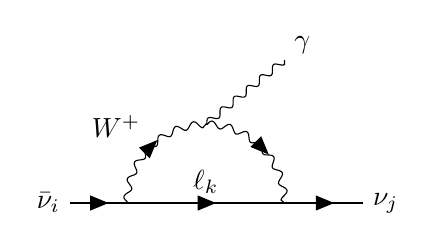
\begin{tikzpicture}
            \begin{feynman}
                \vertex (i1)  {\(\rhn_{i}\)};
                \vertex[right=1cm of i1] (v1) ;
                \vertex[right=1cm of v1] (g1) ;
                \vertex[right=1cm of g1] (v2) ;
                \vertex[above=1cm of g1] (v3) ;
                \vertex[right=1cm of v2] (o1) {\(\nu_{j}\)};
                \vertex[above=1cm of v3] (g2) ;
                \vertex[right=1cm of g2] (o2) {\(\gamma\)};
                \diagram*{
                (i1) -- [fermion] (v1) -- [fermion,edge label=\(\ell_{k}\)](v2) -- [fermion](o1);
                (v1) -- [charged boson,quarter left,looseness=1.0,edge label=\(W^{+}\)] (v3) -- [charged boson,quarter left,looseness=1.0] (v2);
                (v3) -- [boson] (o2);
                };
            \end{feynman}
        \end{tikzpicture}
        \caption{}
    \end{subfigure}
    \begin{subfigure}[b]{0.45\linewidth}
        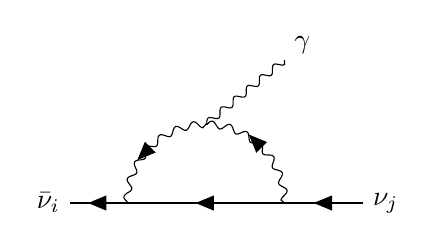
\begin{tikzpicture}
            \begin{feynman}
                \vertex (i1)  {\(\rhn_{i}\)};
                \vertex[right=1cm of i1] (v1) ;
                \vertex[right=1cm of v1] (g1) ;
                \vertex[right=1cm of g1] (v2) ;
                \vertex[above=1cm of g1] (v3) ;
                \vertex[right=1cm of v2] (o1) {\(\nu_{j}\)};
                \vertex[above=1cm of v3] (g2) ;
                \vertex[right=1cm of g2] (o2) {\(\gamma\)};
                \diagram*{
                (o1) -- [fermion] (v2) -- [fermion](v1) -- [fermion](i1);
                (v1) -- [anti charged boson,quarter left,looseness=1.0] (v3) -- [anti charged boson,quarter left,looseness=1.0] (v2);
                (v3) -- [boson] (o2);
                };
            \end{feynman}
        \end{tikzpicture}
        \caption{}
    \end{subfigure}
    \begin{subfigure}[b]{0.45\linewidth}
        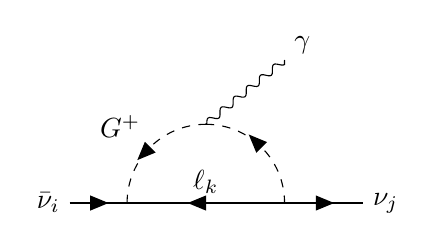
\begin{tikzpicture}
            \begin{feynman}
                \vertex (i1)  {\(\rhn_{i}\)};
                \vertex[right=1cm of i1] (v1) ;
                \vertex[right=1cm of v1] (g1) ;
                \vertex[right=1cm of g1] (v2) ;
                \vertex[above=1cm of g1] (v3) ;
                \vertex[right=1cm of v2] (o1) {\(\nu_{j}\)};
                \vertex[above=1cm of v3] (g2) ;
                \vertex[right=1cm of g2] (o2) {\(\gamma\)};
                \diagram*{
                (i1) -- [fermion] (v1) -- [anti fermion,edge label=\(\ell_{k}\)](v2) -- [fermion](o1);
                (v1) -- [anti charged scalar,quarter left,looseness=1.0,edge label=\(G^{+}\)] (v3) -- [anti charged scalar,quarter left,looseness=1.0] (v2);
                (v3) -- [boson] (o2);
                };
            \end{feynman}
        \end{tikzpicture}
        \caption{}
    \end{subfigure}
    \begin{subfigure}[b]{0.45\linewidth}
        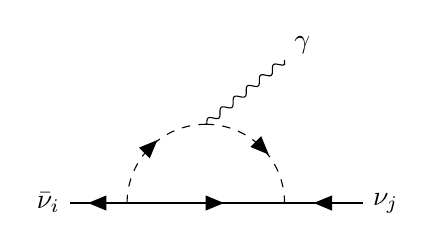
\begin{tikzpicture}
            \begin{feynman}
                \vertex (i1)  {\(\rhn_{i}\)};
                \vertex[right=1cm of i1] (v1) ;
                \vertex[right=1cm of v1] (g1) ;
                \vertex[right=1cm of g1] (v2) ;
                \vertex[above=1cm of g1] (v3) ;
                \vertex[right=1cm of v2] (o1) {\(\nu_{j}\)};
                \vertex[above=1cm of v3] (g2) ;
                \vertex[right=1cm of g2] (o2) {\(\gamma\)};
                \diagram*{
                (o1) -- [fermion] (v2) -- [anti fermion](v1) -- [fermion](i1);
                (v1) -- [charged scalar,quarter left,looseness=1.0] (v3) -- [charged scalar,quarter left,looseness=1.0] (v2);
                (v3) -- [boson] (o2);
                };
            \end{feynman}
        \end{tikzpicture}
        \caption{}
    \end{subfigure}
    \caption{Diagrams contributing to \(\rhn_{i}\to\nu_{j}\gamma\) with photon
        emission from \(W\)-boson.}
    \label{fig:n_to_nu_gamma_w}
\end{figure}

\begin{figure}[ht!]
    \centering
    \begin{subfigure}[b]{0.45\linewidth}
        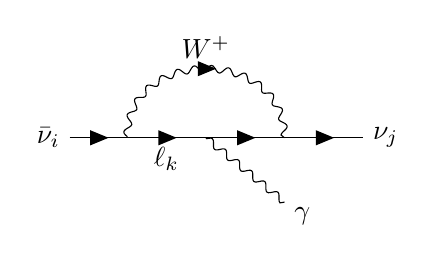
\begin{tikzpicture}
            \begin{feynman}
                \vertex (i1)  {\(\rhn_{i}\)};
                \vertex[right=1cm of i1] (v1) ;
                \vertex[right=1cm of v1] (v2) ;
                \vertex[right=1cm of v2] (v3) ;
                \vertex[right=1cm of v3] (o1) {\(\nu_{j}\)};
                \vertex[below=1cm of v2] (g1) ;
                \vertex[right=1cm of g1] (o2) {\(\gamma\)};
                \diagram*{
                (i1) -- [fermion] (v1) -- [fermion,edge label'=\(\ell_{k}\)](v2) -- [fermion](v3) -- [fermion](o1);
                (v1) -- [charged boson,half left,looseness=1.5,edge label=\(W^{+}\)] (v3) ;
                (v2) -- [boson] (o2);
                };
            \end{feynman}
        \end{tikzpicture}
        \caption{}
    \end{subfigure}
    \begin{subfigure}[b]{0.45\linewidth}
        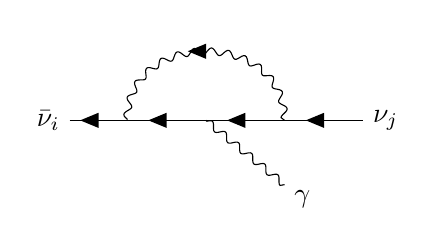
\begin{tikzpicture}
            \begin{feynman}
                \vertex (i1)  {\(\rhn_{i}\)};
                \vertex[right=1cm of i1] (v1) ;
                \vertex[right=1cm of v1] (v2) ;
                \vertex[right=1cm of v2] (v3) ;
                \vertex[right=1cm of v3] (o1) {\(\nu_{j}\)};
                \vertex[below=1cm of v2] (g1) ;
                \vertex[right=1cm of g1] (o2) {\(\gamma\)};
                \diagram*{
                (i1) -- [anti fermion] (v1) -- [anti fermion](v2) -- [anti fermion](v3) -- [anti fermion](o1);
                (v1) -- [anti charged boson,half left,looseness=1.5] (v3) ;
                (v2) -- [boson] (o2);
                };
            \end{feynman}
        \end{tikzpicture}
        \caption{}
    \end{subfigure}
    \begin{subfigure}[b]{0.45\linewidth}
        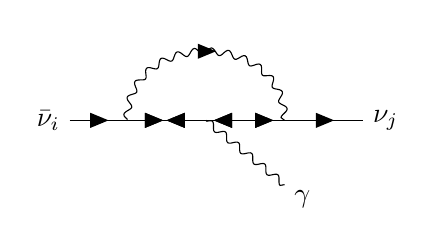
\begin{tikzpicture}
            \begin{feynman}
                \vertex (i1)  {\(\rhn_{i}\)};
                \vertex[right=1cm of i1] (v1) ;
                \vertex[right=1cm of v1] (v2) ;
                \vertex[right=1cm of v2] (v3) ;
                \vertex[right=1cm of v3] (o1) {\(\nu_{j}\)};
                \vertex[below=1cm of v2] (g3) ;
                \vertex[right=1cm of g3] (o2) {\(\gamma\)};
                \diagram*{
                (i1) -- [fermion] (v1) -- [majorana](v2) -- [anti majorana] (v3) -- [fermion](o1);
                (v1) -- [charged boson,half left,looseness=1.5] (v3) ;
                (v2) -- [boson] (o2);
                };
            \end{feynman}
        \end{tikzpicture}
        \caption{}
    \end{subfigure}
    \begin{subfigure}[b]{0.45\linewidth}
        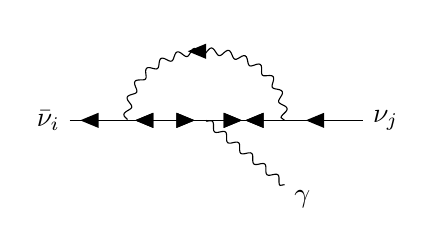
\begin{tikzpicture}
            \begin{feynman}
                \vertex (i1)  {\(\rhn_{i}\)};
                \vertex[right=1cm of i1] (v1) ;
                \vertex[right=1cm of v1] (v2) ;
                \vertex[right=1cm of v2] (v3) ;
                \vertex[right=1cm of v3] (o1) {\(\nu_{j}\)};
                \vertex[below=1cm of v2] (g3) ;
                \vertex[right=1cm of g3] (o2) {\(\gamma\)};
                \diagram*{
                (i1) -- [anti fermion] (v1) -- [anti majorana](v2) -- [majorana] (v3) -- [anti fermion](o1);
                (v1) -- [anti charged boson,half left,looseness=1.5] (v3) ;
                (v2) -- [boson] (o2);
                };
            \end{feynman}
        \end{tikzpicture}
        \caption{}
    \end{subfigure}
    \begin{subfigure}[b]{0.45\linewidth}
        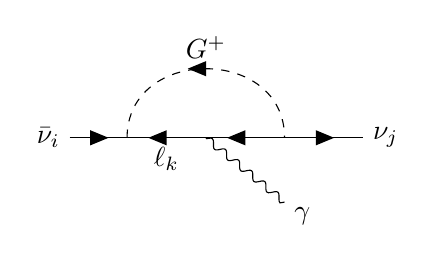
\begin{tikzpicture}
            \begin{feynman}
                \vertex (i1)  {\(\rhn_{i}\)};
                \vertex[right=1cm of i1] (v1) ;
                \vertex[right=1cm of v1] (v2) ;
                \vertex[right=1cm of v2] (v3) ;
                \vertex[right=1cm of v3] (o1) {\(\nu_{j}\)};
                \vertex[below=1cm of v2] (g1) ;
                \vertex[right=1cm of g1] (o2) {\(\gamma\)};
                \diagram*{
                (i1) -- [fermion] (v1) -- [anti fermion,edge label'=\(\ell_{k}\)](v2) -- [anti fermion](v3) -- [fermion](o1);
                (v1) -- [anti charged scalar,half left,looseness=1.5,edge label=\(G^{+}\)] (v3) ;
                (v2) -- [boson] (o2);
                };
            \end{feynman}
        \end{tikzpicture}
        \caption{}
    \end{subfigure}
    \begin{subfigure}[b]{0.45\linewidth}
        \begin{tikzpicture}
            \begin{feynman}
                \vertex (i1)  {\(\rhn_{i}\)};
                \vertex[right=1cm of i1] (v1) ;
                \vertex[right=1cm of v1] (v2) ;
                \vertex[right=1cm of v2] (v3) ;
                \vertex[right=1cm of v3] (o1) {\(\nu_{j}\)};
                \vertex[below=1cm of v2] (g1) ;
                \vertex[right=1cm of g1] (o2) {\(\gamma\)};
                \diagram*{
                (i1) -- [anti fermion] (v1) -- [fermion](v2) -- [fermion](v3) -- [anti fermion](o1);
                (v1) -- [charged scalar,half left,looseness=1.5] (v3) ;
                (v2) -- [boson] (o2);
                };
            \end{feynman}
        \end{tikzpicture}
        \caption{}
    \end{subfigure}
    \begin{subfigure}[b]{0.45\linewidth}
        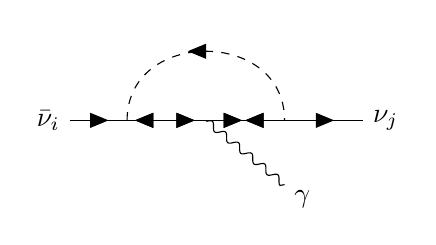
\begin{tikzpicture}
            \begin{feynman}
                \vertex (i1)  {\(\rhn_{i}\)};
                \vertex[right=1cm of i1] (v1) ;
                \vertex[right=1cm of v1] (v2) ;
                \vertex[right=1cm of v2] (v3) ;
                \vertex[right=1cm of v3] (o1) {\(\nu_{j}\)};
                \vertex[below=1cm of v2] (g3) ;
                \vertex[right=1cm of g3] (o2) {\(\gamma\)};
                \diagram*{
                (i1) -- [fermion] (v1) -- [anti majorana](v2) -- [majorana] (v3) -- [fermion](o1);
                (v1) -- [anti charged scalar,half left,looseness=1.5] (v3) ;
                (v2) -- [boson] (o2);
                };
            \end{feynman}
        \end{tikzpicture}
        \caption{}
    \end{subfigure}
    \begin{subfigure}[b]{0.45\linewidth}
        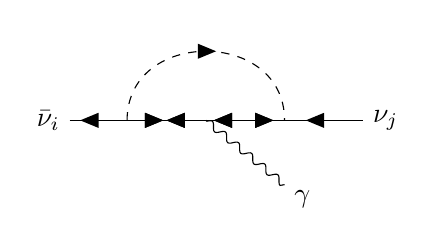
\begin{tikzpicture}
            \begin{feynman}
                \vertex (i1)  {\(\rhn_{i}\)};
                \vertex[right=1cm of i1] (v1) ;
                \vertex[right=1cm of v1] (v2) ;
                \vertex[right=1cm of v2] (v3) ;
                \vertex[right=1cm of v3] (o1) {\(\nu_{j}\)};
                \vertex[below=1cm of v2] (g3) ;
                \vertex[right=1cm of g3] (o2) {\(\gamma\)};
                \diagram*{
                (i1) -- [anti fermion] (v1) -- [majorana](v2) -- [anti majorana] (v3) -- [anti fermion](o1);
                (v1) -- [charged scalar,half left,looseness=1.5] (v3) ;
                (v2) -- [boson] (o2);
                };
            \end{feynman}
        \end{tikzpicture}
        \caption{}
    \end{subfigure}
    \caption{Diagrams contributing to \(\rhn_{i}\to\nu_{j}\gamma\) with photon
        emission from charged lepton. Note diagrams use two-component spinors
        with (c), (d), (g) and (f) representing charged lepton mass insertions.}
    \label{fig:n_to_nu_gamma_ell}
\end{figure}

We will denote the \(W^{+}W^{-}\gamma\) vertex as \(V^{\alpha\beta\mu}(p^{+}_{\alpha},p^{-}_{\beta},p^{\gamma}_{\mu})\),
given by:
\begin{align}
	V_{WW\gamma}^{\alpha\beta\mu}(p^{+}_{\alpha},p^{-}_{\beta},p^{\gamma}_{\mu}) =
	ie\qty[
		g^{\alpha\beta}\qty(p^{-}-p^{+})_{\mu} +
		g^{\alpha\mu}\qty(p^{+}-p^{\gamma})_{\beta} +
		g^{\beta\mu}\qty(p^{\gamma}-p^{-})_{\alpha}
	]
\end{align}
We denote the \(G^{+}G^{-}\gamma\) vertex as \(V^{\mu}(p^{+},p^{-})\), given by:
\begin{align}
	V_{GG\gamma}^{\mu}(p^{+},p^{-}) = ie\qty(p^{+} - p^{-})_{\mu}
\end{align}
Note that \(V_{WW\gamma}^{\alpha\beta\mu}(p^{+}_{\alpha},p^{-}_{\beta},p^{\gamma}_{\mu}) = -V_{WW\gamma}^{\beta\alpha\mu}(p^{-}_{\alpha},p^{+}_{\beta},p^{\gamma}_{\mu})\)
and \(V_{GG\gamma}^{\mu}(p^{+},p^{-}) = - V_{GG\gamma}^{\mu}(p^{-},p^{+})\).
We use \(\Delta\) for a propagator. For example:
\begin{align}
	\Delta^{\mu\nu}_{W}(p) & = \frac{i}{p^2-M_{W}^{2}+i\epsilon}\qty(-g^{\mu\nu} + (1-\xi)\frac{p^{\mu}p^{\nu}}{p^{2}-\xi M_{W}^{2}}) \\
	\Delta^{G}(p)          & = \frac{i}{p^2-\xi M_{W}^{2}+i\epsilon}
\end{align}
In addition, we denote the neutrino interactions as:
\begin{align}
	V^{\mu}_{W\nu_{i}\ell_{j}}  & \equiv A = \frac{e}{\sqrt{2}\sw}\qty(\bm{\cK}_{L})^{ij}\bar{\sigma}_{\mu}     \\
	V^{\mu}_{W\rhn_{i}\ell_{j}} & \equiv B = \frac{e}{\sqrt{2}\sw}\qty(\bm{\cK}_{R})^{ij}\bar{\sigma}_{\mu}     \\
	V_{G\nu_{i}\ell_{j}}        & \equiv \tilde{A} =  \frac{e}{\sqrt{2}\sw}\qty(\hat{\bm{m}}_{D}\OmegaVVb)^{ij} \\
	V_{G\rhn_{i}\ell_{j}}       & \equiv \tilde{B} = \frac{e}{\sqrt{2}\sw}\qty(\hat{\bm{m}}_{D}\OmegaVNb)^{ij}
\end{align}

% ============================================================================
% ---- W-Emission Diagrams ---------------------------------------------------
% ============================================================================

The amplitude of the diagrams with \(W\)-bosons in \FigRef{fig:n_to_nu_gamma_w} are given by
\begin{align}
	i\cA^{(a)}_{1}
	 & =
	-i\qty(A^{*}B)
	\int\frac{\dd[4]{\ell}}{(2\pi)^{4}}
	\frac{x_{\nu}^{\dagger}(q)\bar{\sigma}_{\mu}\qty(\ell\cdot\sigma)\bar{\sigma}_{\nu}x_{\rhn}(p)}{\ell^{2}-m_{\ell_{k}}^{2}} \\
	 & \quad \times
	\Delta^{\nu\rho}_{W}(p-\ell)
	\Delta^{\lambda\mu}_{W}(\ell-q)
	V^{\rho\lambda\alpha}_{WW\gamma}(p-\ell,\ell-q,-k)
	\epsilon^{*}_{\alpha}(k)
	\notag                                                                                                                     \\
	%--------------------------
	i\cA^{(b)}_{1}
	 & =
	i\qty(AB^{*})
	\int\frac{\dd[4]{\ell}}{(2\pi)^{4}}
	\frac{y_{\nu}(q)\sigma_{\mu}\qty(\ell\cdot\bar{\sigma})\sigma_{\nu}y^{\dagger}_{\rhn}(p) }{\ell^{2}-m_{\ell_{k}}^{2}}      \\
	 & \quad \times
	\Delta^{\nu\rho}_{W}(p-\ell)
	\Delta^{\lambda\mu}_{W}(\ell-q)
	V^{\rho\lambda\alpha}_{WW\gamma}(p-\ell,\ell-q,-k)
	\epsilon^{*}_{\alpha}(k)
	\notag
\end{align}

% ============================================================================
% ---- G-Emission Diagrams ---------------------------------------------------
% ============================================================================

The amplitude of the diagrams with Goldstones in \FigRef{fig:n_to_nu_gamma_w} are given by
\begin{align}
	i\cA^{(c)}_{1}
	 & =
	-i\qty(\tilde{A}\tilde{B}^{*})
	\int\frac{\dd[4]{\ell}}{(2\pi)^{4}}
	\frac{x_{\nu}^{\dagger}(q)\qty[\ell\cdot\bar{\sigma}]x_{\rhn}(p)}{\ell^{2}-m_{\ell_{k}}^{2}}
	\\
	 & \quad \times
	\Delta^{G}(p-\ell)
	\Delta^{G}(\ell-q)
	V^{\alpha}_{GG\gamma}(p-\ell,\ell-q)
	\epsilon^{*}_{\alpha}(k)
	\notag          \\
	%--------------------------
	i\cA^{(d)}_{1}
	 & =
	i\qty(\tilde{A}^{*}\tilde{B})
	\int\frac{\dd[4]{\ell}}{(2\pi)^{4}}
	\frac{y_{\nu}(q)\qty[\ell\cdot\sigma]y^{\dagger}_{\rhn}(p)}{\ell^{2}-m_{\ell_{k}}^{2}}
	\\
	 & \quad \times
	\Delta^{G}(p-\ell)
	\Delta^{G}(\ell-q)
	V^{\alpha}_{GG\gamma}(p-\ell,\ell-q)
	\epsilon^{*}_{\alpha}(k)
	\notag
\end{align}


% ============================================================================
% ---- L-Emission Diagrams with W --------------------------------------------
% ============================================================================

The amplitudes for the diagrams with \(W\)-bosons in \FigRef{fig:n_to_nu_gamma_ell} are given by
\begin{align}
	i\cA^{(a)}_{2}
	 & =
	-ieA^{*}B
	\int\frac{\dd[4]{\ell}}{(2\pi)^{4}}
	\frac{
	x_{\nu}^{\dagger}(q)
	\bar{\sigma}_{\mu}
	\qty[\qty(q-\ell)\cdot\sigma]
	\bar{\sigma}_{\alpha}
	\qty[\qty(p-\ell)\cdot\sigma]
	\bar{\sigma}_{\nu}
	x_{\rhn}(p)
	}{
	\qty[\qty(p-\ell)^{2}-m_{\ell_{k}}^{2}]\qty[\qty(q-\ell)^{2}-m_{\ell_{k}}^{2}]
	}
	\Delta^{\mu\nu}_{W}(\ell)
	\epsilon^{*}_{\alpha}(k)
	\\
	%--------------------------
	i\cA^{(b)}_{2}
	 & =
	ieAB^{*}
	\int\frac{\dd[4]{\ell}}{(2\pi)^{4}}
	\frac{
	y_{\nu}(q)
	\sigma_{\mu}
	\qty[\qty(q-\ell)\cdot\bar{\sigma}]
	\sigma_{\alpha}
	\qty[\qty(p-\ell)\cdot\bar{\sigma}]
	\sigma_{\nu}
	y_{\rhn}^{\dagger}(p)
	}{
	\qty[\qty(q-\ell)^{2}-m_{\ell_{k}}^{2}]\qty[\qty(p-\ell)^{2}-m_{\ell_{k}}^{2}]
	}
	\Delta^{\mu\nu}_{W}(\ell)
	\epsilon^{*}_{\alpha}(k)
	\\
	i\cA^{(c)}_{2}
	 & =
	-ieA^{*}B m^{2}_{\ell_{k}}
	\int\frac{\dd[4]{\ell}}{(2\pi)^{4}}
	\frac{
	x_{\nu}^{\dagger}(q)
	\bar{\sigma}_{\mu}\sigma_{\alpha}\bar{\sigma}_{\nu}
	x_{\rhn}(p)
	}{
	\qty[\qty(q-\ell)^{2}-m_{\ell_{k}}^{2}]\qty[\qty(p-\ell)^{2}-m_{\ell_{k}}^{2}]
	}
	\Delta^{\mu\nu}_{W}(\ell)
	\epsilon^{*}_{\alpha}(k)
	\\
	i\cA^{(d)}_{2}
	 & =
	ieAB^{*}m^{2}_{\ell_{k}}
	\int\frac{\dd[4]{\ell}}{(2\pi)^{4}}
	\frac{
	y_{\nu}(q)
	\sigma_{\mu}
	\bar{\sigma}_{\alpha}
	\sigma_{\nu}
	y_{\rhn}^{\dagger}(p)
	}{
	\qty[\qty(q-\ell)^{2}-m_{\ell_{k}}^{2}]\qty[\qty(p-\ell)^{2}-m_{\ell_{k}}^{2}]
	}
	\Delta^{\mu\nu}_{W}(\ell)
	\epsilon^{*}_{\alpha}(k)
\end{align}


% ============================================================================
% ---- L-Emission Diagrams with G --------------------------------------------
% ============================================================================

The amplitudes for the diagrams with Goldstones in \FigRef{fig:n_to_nu_gamma_ell} are given by
\begin{align}
	i\cA^{(e)}_{2}
	 & =
	-ie\tilde{A}\tilde{B}^{*}
	\int\frac{\dd[4]{\ell}}{(2\pi)^{4}}
	\frac{
	x_{\nu}^{\dagger}(q)
	\qty[\qty(q-\ell)\cdot\bar{\sigma}]\sigma_{\alpha}\qty[\qty(p-\ell)\cdot\bar{\sigma}]
	x_{\rhn}(p)
	}{
	\qty[\qty(q-\ell)^{2}-m_{\ell_{k}}^{2}]\qty[\qty(p-\ell)^{2}-m_{\ell_{k}}^{2}]
	}
	\Delta^{G}(\ell)
	\epsilon^{*}_{\alpha}(k)
	\\
	%--------------------------
	i\cA^{(f)}_{2}
	 & =
	-ie\tilde{A}^{*}\tilde{B}
	\int\frac{\dd[4]{\ell}}{(2\pi)^{4}}
	\frac{
	y_{\nu}(q)
	\qty[\qty(q-\ell)\cdot\sigma]\bar{\sigma}_{\alpha}\qty[\qty(p-\ell)\cdot\sigma]
	y_{\rhn}^{\dagger}(p)
	}{
	\qty[\qty(q-\ell)^{2}-m_{\ell_{k}}^{2}]\qty[\qty(p-\ell)^{2}-m_{\ell_{k}}^{2}]
	}
	\Delta^{G}(\ell)
	\epsilon^{*}_{\alpha}(k)
	\\
	i\cA^{(g)}_{2}
	 & =
	ie\tilde{A}\tilde{B}^{*}m^{2}_{\ell_{k}}
	\int\frac{\dd[4]{\ell}}{(2\pi)^{4}}
	\frac{
	x_{\nu}^{\dagger}(q)\bar{\sigma}_{\alpha}x_{\rhn}(p)
	}{
	\qty[\qty(q-\ell)^{2}-m_{\ell_{k}}^{2}]\qty[\qty(p-\ell)^{2}-m_{\ell_{k}}^{2}]
	}
	\Delta^{G}(\ell)
	\epsilon^{*}_{\alpha}(k)
	\\
	i\cA^{(h)}_{2}
	 & =
	-ie\tilde{A}^{*}\tilde{B}m^{2}_{\ell_{k}}
	\int\frac{\dd[4]{\ell}}{(2\pi)^{4}}
	\frac{
	y_{\nu}(q)\sigma_{\alpha}y_{\rhn}^{\dagger}(p)
	}{
	\qty[\qty(q-\ell)^{2}-m_{\ell_{k}}^{2}]\qty[\qty(p-\ell)^{2}-m_{\ell_{k}}^{2}]
	}
	\Delta^{G}(\ell)
	\epsilon^{*}_{\alpha}(k)
\end{align}



\subsubsection{\texorpdfstring{\(\rhn_{i}\to\nu_{j}\pi^{0},\nu_{j}\eta\)}{RH-Neutrino to LH-Neutrino and Neutral Pion}}

The relavent interactions for \(\rhn_{i}\to\nu_{j}\pi^{0}\) stem from
\begin{align}
    \cL_{4F} & = -\frac{4\gf\fpi}{2\cw^{2}\sqrt{2}}\qty(\partial_{\mu}\piz)
    \qty(\qty(\OmegaVVb^{\dagger}\OmegaVNb)^{ij}
    \nu_{i}^{\dagger}
    \bar{\sigma}_{\mu}
    \rhn_{j}
    +\qty(\OmegaVNb^{\dagger}\OmegaVVb)^{ij}\rhn_{i}^{\dagger}
    \bar{\sigma}_{\mu}
    \nu_{j}
    )
\end{align}
Thus, the amplitude is given by:
\begin{align}
    i\cM\qty(\rhn_{i}\to\nu_{j}\pi^{0})
    =
    -i\frac{\sqrt{2}\gf\fpi}{\cw^{2}}\qty(i p^{\mu}_{\piz})
    \qty[
    gx^{\dagger}_{\nu}\bar{\sigma}_{\mu}x_{\rhn}
    -
    g^{*}y^{\dagger}_{\rhn}\bar{\sigma}_{\mu}y_{\nu}
    ]
\end{align}
where \(g\equiv \qty(\OmegaVVb^{\dagger}\OmegaVNb)^{ij}\).
Squaring and summing over spins yields:
\begin{align}
    \frac{1}{2}\sum_{\mathrm{spins}}\qty|\cM\qty(\rhn_{i}\to\nu_{j}\pi^{0})|^{2}
     & =
    \frac{2\gf^{2}\fpi^{2}}{\cw^{4}}
    \bigg{[}
    |g|^{2}\qty(\qty(m_{\rhn_{i}}^{2}-m_{\nu_{j}}^{2})^{2}
    - m_{\piz}^{2}\qty(m_{\rhn_{i}}^{2}+m_{\nu_{j}}^{2})) \\
     & \qquad\qquad\qquad
    -4\Re(g^2)m_{\rhn_{i}}m_{\nu_{j}}m_{\piz}^{2}
    \bigg{]}\notag
\end{align}
and thus, the partial width is:
\begin{align}
    \Gamma\qty(\rhn_{i}\to\nu_{j}\pi^{0})
    =
    \frac{\gf^{2}\fpi^{2}m^{3}_{\rhn_{i}}}{8\pi \cw^{4}}
    \lambda^{1/2}(1,\beta_{\nu_{j}}^2,\beta_{\pi}^{2})
     &
    \bigg{[}
    |g|^{2}\qty(\qty(1-\beta_{\nu_{j}}^{2})^{2}
    - \beta_{\piz}^{2}\qty(1+\beta_{\nu_{j}}^{2})) \\
     & \quad
    -4\Re(g^2)\beta_{\nu_{j}}\beta_{\piz}^{2}
    \bigg{]}\notag
\end{align}
The result for \(\rhn_{i}\to\nu_{j}\eta\) is identical but has an extra factor of
\(1/3\)
\begin{align}
    \Gamma\qty(\rhn_{i}\to\nu_{j}\eta)
    =
    \frac{\gf^{2}\fpi^{2}m^{3}_{\rhn_{i}}}{24\pi \cw^{4}}
    \lambda^{1/2}(1,\beta_{\nu_{j}}^2,\beta_{\eta}^{2})
     &
    \bigg{[}
    |g|^{2}\qty(\qty(1-\beta_{\nu_{j}}^{2})^{2}
    - \beta_{\eta}^{2}\qty(1+\beta_{\nu_{j}}^{2})) \\
     & \quad
    -4\Re(g^2)\beta_{\nu_{j}}\beta_{\eta}^{2}
    \bigg{]}\notag
\end{align}




\subsubsection{\texorpdfstring{\(\rhn_{i}\to\ell_{j}\pip,\ell_{j}\kp\)}{RH-Neutrino to Charged Lepton and Charged Pion}}

The relavent interactions for \(\rhn_{i}\to\ell_{j}\pip\) stem from
\begin{align}
    \cL_{4F} & = -2\gf\fpi\vud\qty(\partial_{\mu}\pim)
    \qty(\OmegaVNb)^{ji}
    \ell_{j}^{\dagger}
    \bar{\sigma}_{\mu}
    \rhn_{i}
\end{align}
Thus, the amplitude is given by:
\begin{align}
    i\cM\qty(\rhn_{i}\to\ell_{j}\pip)
    =
    -2g\gf\fpi\vud\qty(ip_{\pip})
    x^{\dagger}_{\ell}\bar{\sigma}_{\mu}x_{\rhn}
\end{align}
where \(g\equiv \qty(\OmegaVNb)^{ji}\).
Squaring and summing over spins yields:
\begin{align}
    \frac{1}{2}\sum_{\mathrm{spins}}\qty|\cM\qty(\rhn_{i}\to\ell_{j}\pip)|^{2}
     & =
    2\qty|g|^{2}\gf^{2}\fpi^{2}\qty|\vud|^{2}
    \qty[\qty(m_{\rhn_{i}}^{2}-m_{\ell_{j}}^{2})^{2}
        - m_{\pip}^{2}\qty(m_{\rhn_{i}}^{2}+m_{\ell_{j}}^{2})]
\end{align}
and thus, the partial width is:
\begin{align}
    \Gamma\qty(\rhn_{i}\to\ell_{j}\pip)
    =
    \frac{\qty|g|^{2}\gf^{2}\fpi^{2}\qty|\vud|^{2}m^{3}_{\rhn_{i}}}{8\pi}
    \lambda^{1/2}(1,\beta_{\ell}^2,\beta_{\pip}^{2})
    \qty[\qty(1-\beta_{\ell_{j}}^{2})^{2}
        - \beta_{\pip}^{2}\qty(1+\beta_{\ell_{j}}^{2})]
\end{align}
The result for \(\rhn_{i}\to\ell_{j}K^{+}\) is obtained from the above with
the replacements \(V_{ud}\to V_{us}\) and \(\beta_{\pip}\to\beta_{\kp}\)
\begin{align}
    \Gamma\qty(\rhn_{i}\to\ell_{j}\kp)
    =
    \frac{\qty|g|^{2}\gf^{2}\fpi^{2}\qty|\vus|^{2}m^{3}_{\rhn_{i}}}{8\pi}
    \lambda^{1/2}(1,\beta_{\ell}^2,\beta_{\kp}^{2})
    \qty[\qty(1-\beta_{\ell_{j}}^{2})^{2}
        - \beta_{\kp}^{2}\qty(1+\beta_{\ell_{j}}^{2})]
\end{align}


\subsection{Three-Body Partial Widths}
Here we compute the partial widths of the general RH neutrino model into three-body
final states.


\subsubsection{\texorpdfstring{\(\rhn_{i}\to\nu_{j}q\bar{q}\)}{RH-Neutrino to LH-Neutrino and Quarks}}
The amplitude for \(\rhn_{i}(P) \to \nu_{j}(p_{\nu}) + q(p_{q}) + \bar{q}(p_{\bar{q}})\), where
\(q \in \qty{u,c,t,d,s,b}\) is a SM quark, contains a Z and a Higgs exchanged diagram. The diagrams are given by:
\begin{align}
    i\cM
     & =
    \qty[iG_{ij}y_{\nu}x_{\rhn} + iG^{*}_{ij}x^{\dagger}_{\nu}y^{\dagger}_{\rhn}]
    \qty(i\Delta_{h})
    \qty(-i\frac{m_{q}}{v})
    \qty[x^{\dagger}_{q}x^{\dagger}_{\bar{q}} + y_{u}y_{\bar{q}}] \\
     & \quad +
    \qty(i\tilde{G}_{ij})
    \qty[x^{\dagger}_{\nu}\bar{\sigma}^{\mu}x_{\rhn} - y^{\dagger}_{\rhn}\bar{\sigma}^{\mu}y_{\nu}]
    \qty(i\Delta^{\mu\nu}_{Z})
    \qty[ig^{q}_{L}x^{\dagger}_{q}\bar{\sigma}^{\mu}y_{\bar{q}} -ig^{q}_{R}x^{\dagger}_{\bar{q}}\bar{\sigma}^{\mu}y_{q}]
\end{align}
where \(G_{ij} = \qty(\OmegaNNb^{T}\hat{\bm{m}}\OmegaNVb)_{ij}\),
\(\tilde{G}_{ij} = (e/c_{W}s_{W})\qty(\OmegaVVb^{\dagger}\OmegaVN)_{ij}\) and the left and right handed
quark couplings to the Z are:
\begin{align}
    g^{q}_{L} & = \frac{e}{c_{W}s_{W}}\qty(T^{3}_{q} - s^{2}_{W}Q_{q}), &
    g^{q}_{R} & = \frac{e s_{W}}{c_{W}}Q_{q}
\end{align}
with \(T^{3}_{u} = 1/2, Q_{u}=2/3\) for up-type quarks and
\(T^{3}_{d} = -1/2, Q_{d}=-1/3\) for down-type quarks.
\(\Delta_{h}\) and \(\Delta^{\mu\nu}_{Z}\) are propagators for the Higgs and
Z-boson (in the unitary gauge) given by:
\begin{align}
    \Delta_{h}(p)
                                                   & =
    \frac{1}{p^2 - M^{2}_{h} + i M_{h}\Gamma_{h}}, &
    \Delta^{\mu\nu}_{Z}(p)
                                                   & =
    \frac{1}{p^2 - M^{2}_{Z} + i M_{Z}\Gamma_{Z}}
    \qty(-g^{\mu\nu} + \frac{p^{\mu}p^{\nu}}{M^{2}_{Z}})
\end{align}
Squaring and summing over spins, we find:
\begin{align}
    \frac{1}{2}\sum_{\mathrm{spins}}\qty|\cM|^2
     & =
    \frac{1}{2}\qty(
    N Q \qty|\Delta_{h}|^{2}
    + \qty[N_{\mu}Q_{\nu}\Delta^{\mu\nu}_{Z}\qty(\Delta_{H})^{*} + \mathrm{c.c}]
    + N_{\mu\alpha} Q_{\nu\beta}\Delta_{Z}^{\mu\nu}\qty(\Delta_{Z}^{\alpha\beta})^{*}
    )
\end{align}
where
\begin{align}
    N
     & =
    2\qty(
    \Re(G^{2}_{ij})m_{\nu_{j}}m_{\rhn_{i}}+4\qty|G_{ij}|^{2}\qty(P\cdot p_{\nu})
    )
    \\
    Q
     & = -\frac{4m^{2}_{u_{k}}}{v^{2}}\qty(m^{2}_{u_{k}} - p_{u}p_{\bar{u}})
    \\
    N^{\mu}
     & =
    \frac{2e}{c_{W}s_{W}}\qty(
    \mathrm{Im}\qty(G_{ij}\qty(\tilde{G}_{ij})^{*})m_{\nu_{j}}P^{\mu}
    - m_{\rhn_{i}}\Im(G_{ij}\tilde{G}_{ij})p^{\mu}_{\nu}
    )
    \\
    Q^{\mu}
     & =
    \frac{2m_{u_{k}}^{2}}{v}\qty(g_{L,q}-g_{R,q})(p^{\mu}_{u}-p^{\mu}_{\bar{u}})
    \\
    N^{\mu\alpha}
     & =
    -2\qty(
    2\Re(\tilde{G}_{ij})m_{\nu_{j}}m_{\rhn_{i}}g^{\mu\alpha}
    -2\qty|\tilde{G}_{ij}|^{2}\qty(
    P^{\alpha}p^{\mu}_{\nu} +
    P^{\mu}p^{\alpha}_{\nu}-\qty(P\cdot p_{\nu})g^{\mu\alpha}
    )
    )                                                                        \\
    Q^{\nu\beta}
     & =
    2\qty(g^{2}_{L,q} + g^{2}_{R,q})
    \qty(
    p^{\nu}_{u}p^{\beta}_{\bar{u}} +
    p^{\beta}_{u}p^{\nu}_{\bar{u}}
    )
    -2\qty(\qty(g^{2}_{L,q} + g^{2}_{R,q})\qty(p_{u}\cdot p_{\bar{u}})
    -2g_{L,q}g_{R,q}m^{2}_{u_{k}}
    )
\end{align}




% The bibliography will probably be heavily edited during typesetting.
% We'll parse it and, using the arxiv number or the journal data, will
% query inspire, trying to verify the data (this will probalby spot
% eventual typos) and retrive the document DOI and eventual errata.
% We however suggest to always provide author, title and journal data:
% in short all the informations that clearly identify a document.
\bibliographystyle{JHEP}
\bibliography{DMRHN}


% Please avoid comments such as "For a review'', "For some examples",
% "and references therein" or move them in the text. In general,
% please leave only references in the bibliography and move all
% accessory text in footnotes.

% Also, please have only one work for each \bibitem.

\end{document}
